%%%%%%%%%%%%%%%%%%%%%%%%%%%%%%%%%%%%%%%%%%%%%%%%%%%%%%%%%%%%%%%%%%%%%%%%%%
%%%%%%%%%%%%%%%%%%%%%%%%%%%%%%%%%%%%%%%%%%%%%%%%%%%%%%%%%%%%%%%%%%%%%%%%%%
\clearpage{}
\section{Signal and background expectations from CMS simulation}
\label{sec:MCexpectations}
% ---- ---- ---- ---- ---- ---- ---- ---- ---- ---- --

In order to compare the Monte Carlo processes with observed data, we first normalize each sample to the observed integrated luminosity for both the muon and electron channel of the full 2012 dataset, which, after single lepton triggers, is 19.297 $\textnormal{fb}^{-1}$ and 19.166 $\textnormal{fb}^{-1}$, respectively.  To do this, we use the following calculation

\begin{center}
\begin{equation}\label{normalize}
N_{events} = K \cdot \sigma \cdot \cal{L} \cdot \cal{A} \cdot \varepsilon_{MC} \cdot SF
\end{equation}
\end{center}

where $N_{events}$ is the expected event yield for each Monte Carlo
process after event selection, $K$ is the NLO:LO K-factor, $\sigma$ is
the theoretical cross section for each Monte Carlo process, $\cal{L}$
is the observed integrated luminosity, $\cal{A} \cdot
\varepsilon_{MC}$ is the Monte Carlo process's acceptance times event
selection efficiency, and SF is the efficiency scale factor for data
and Monte Carlo ($\frac{\varepsilon_{data}}{\varepsilon_{MC}}$).

We use the functional fit to the photon fake rate discussed in section~\ref{sec:photon} to estimate the number of observed data events that are from the photon-faking jet background.  
%Since the fit was applied to the fake ratio, or $\frac{fake photon candidates}{true photon candidates}$, then after algebraic reordering the photon $p_{T}$-dependent fake rate function for the barrel region is described by

%\begin{center}
%\begin{equation}\label{fakerate}
%\frac{fake photon candidates}{all photon candidates} = [1 + (0.0345868 + \frac{1.44022 x 10^{4}}{p_{T}^{2.89994}})^{-1}]^{-1}
%\end{equation}
%\end{center}

%where the function can only be used for photon $p_{T}$ greater than 30 GeV.  We simply apply this function as a photon $p_{T}$-dependent scale factor to all observed data events that pass event selection cuts to estimate the fake photon contamination.  

Figures~\ref{photonplots}-\ref{eldijetplots} are Data and Monte Carlo comparison plots for various event kinematical distributions.

\begin{figure}[b]
\begin{center}
\subfigure[]{
   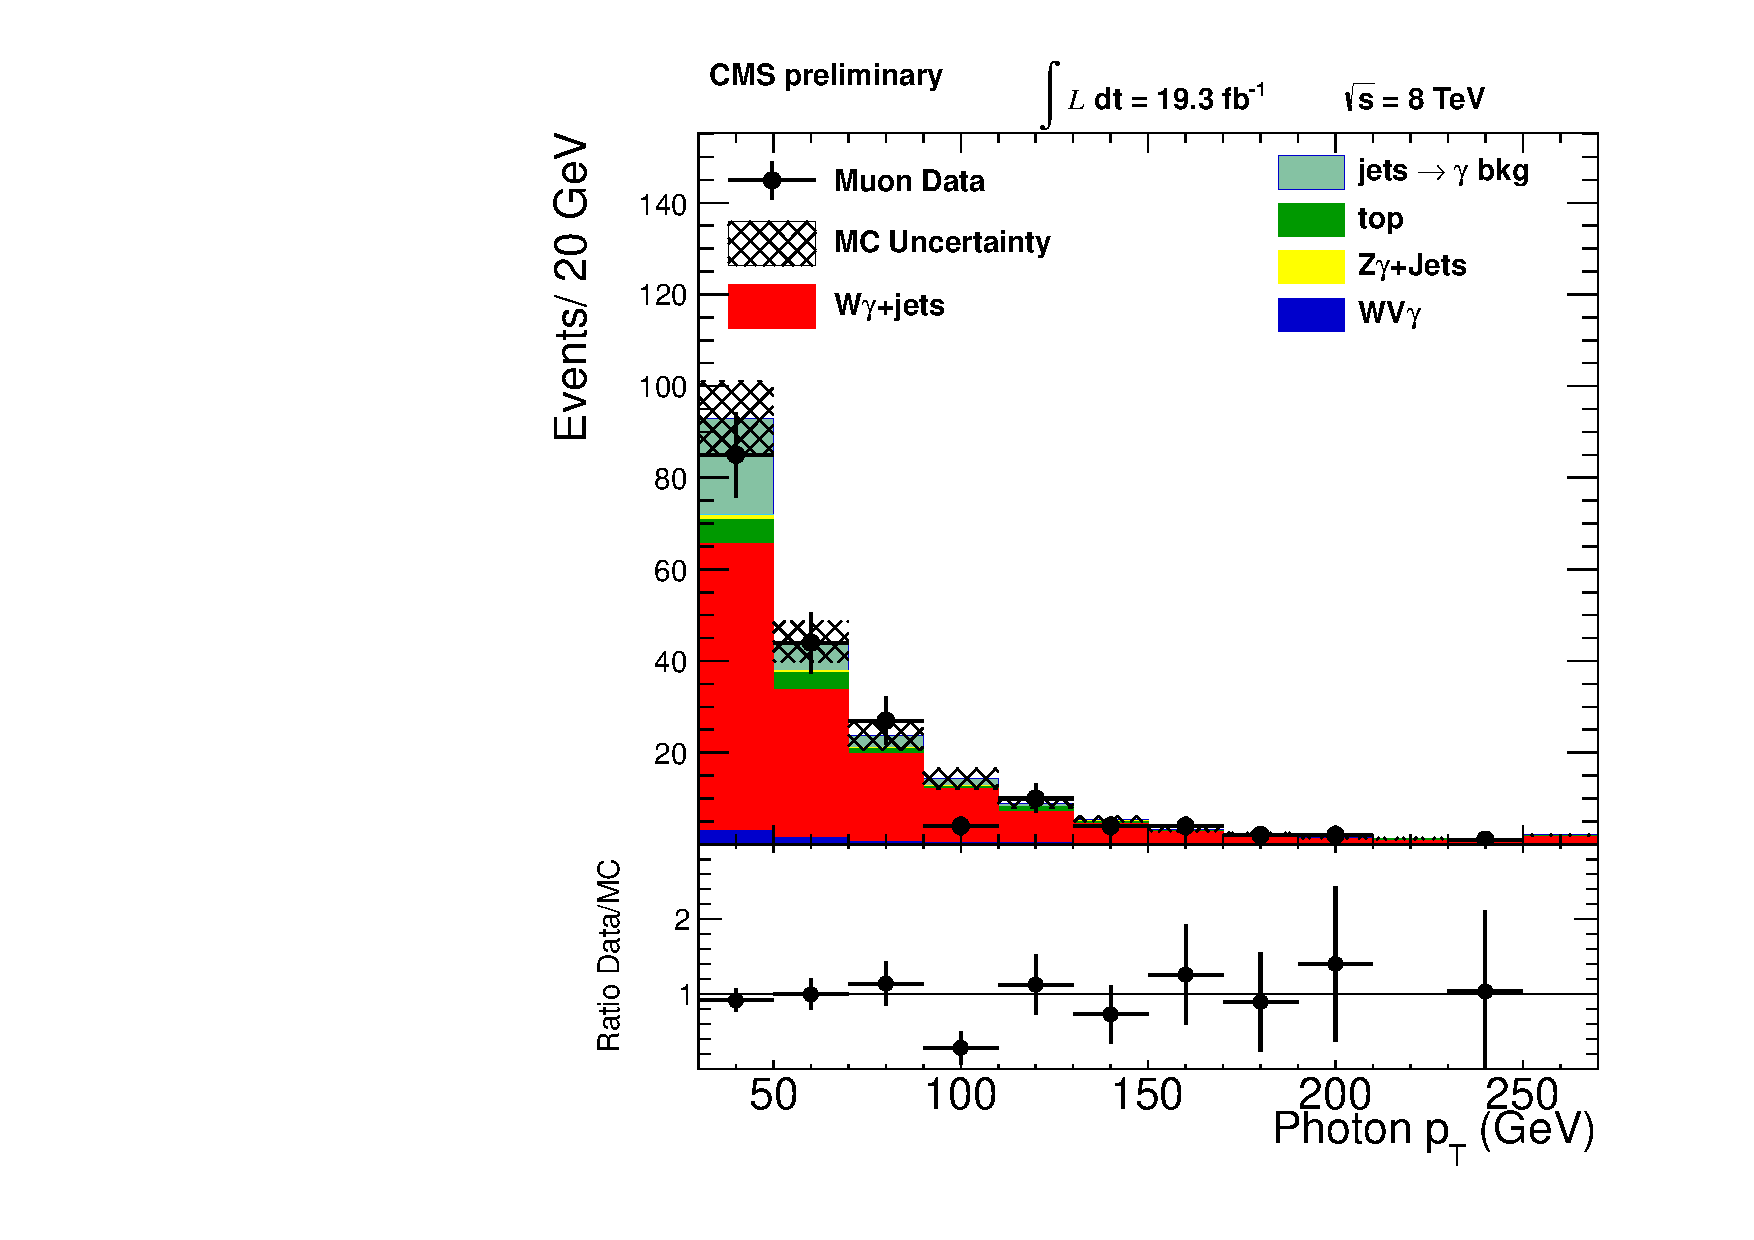
\includegraphics[width=.32\textwidth]{figs/mu_Photon_pt.pdf}
}
\subfigure[]{
   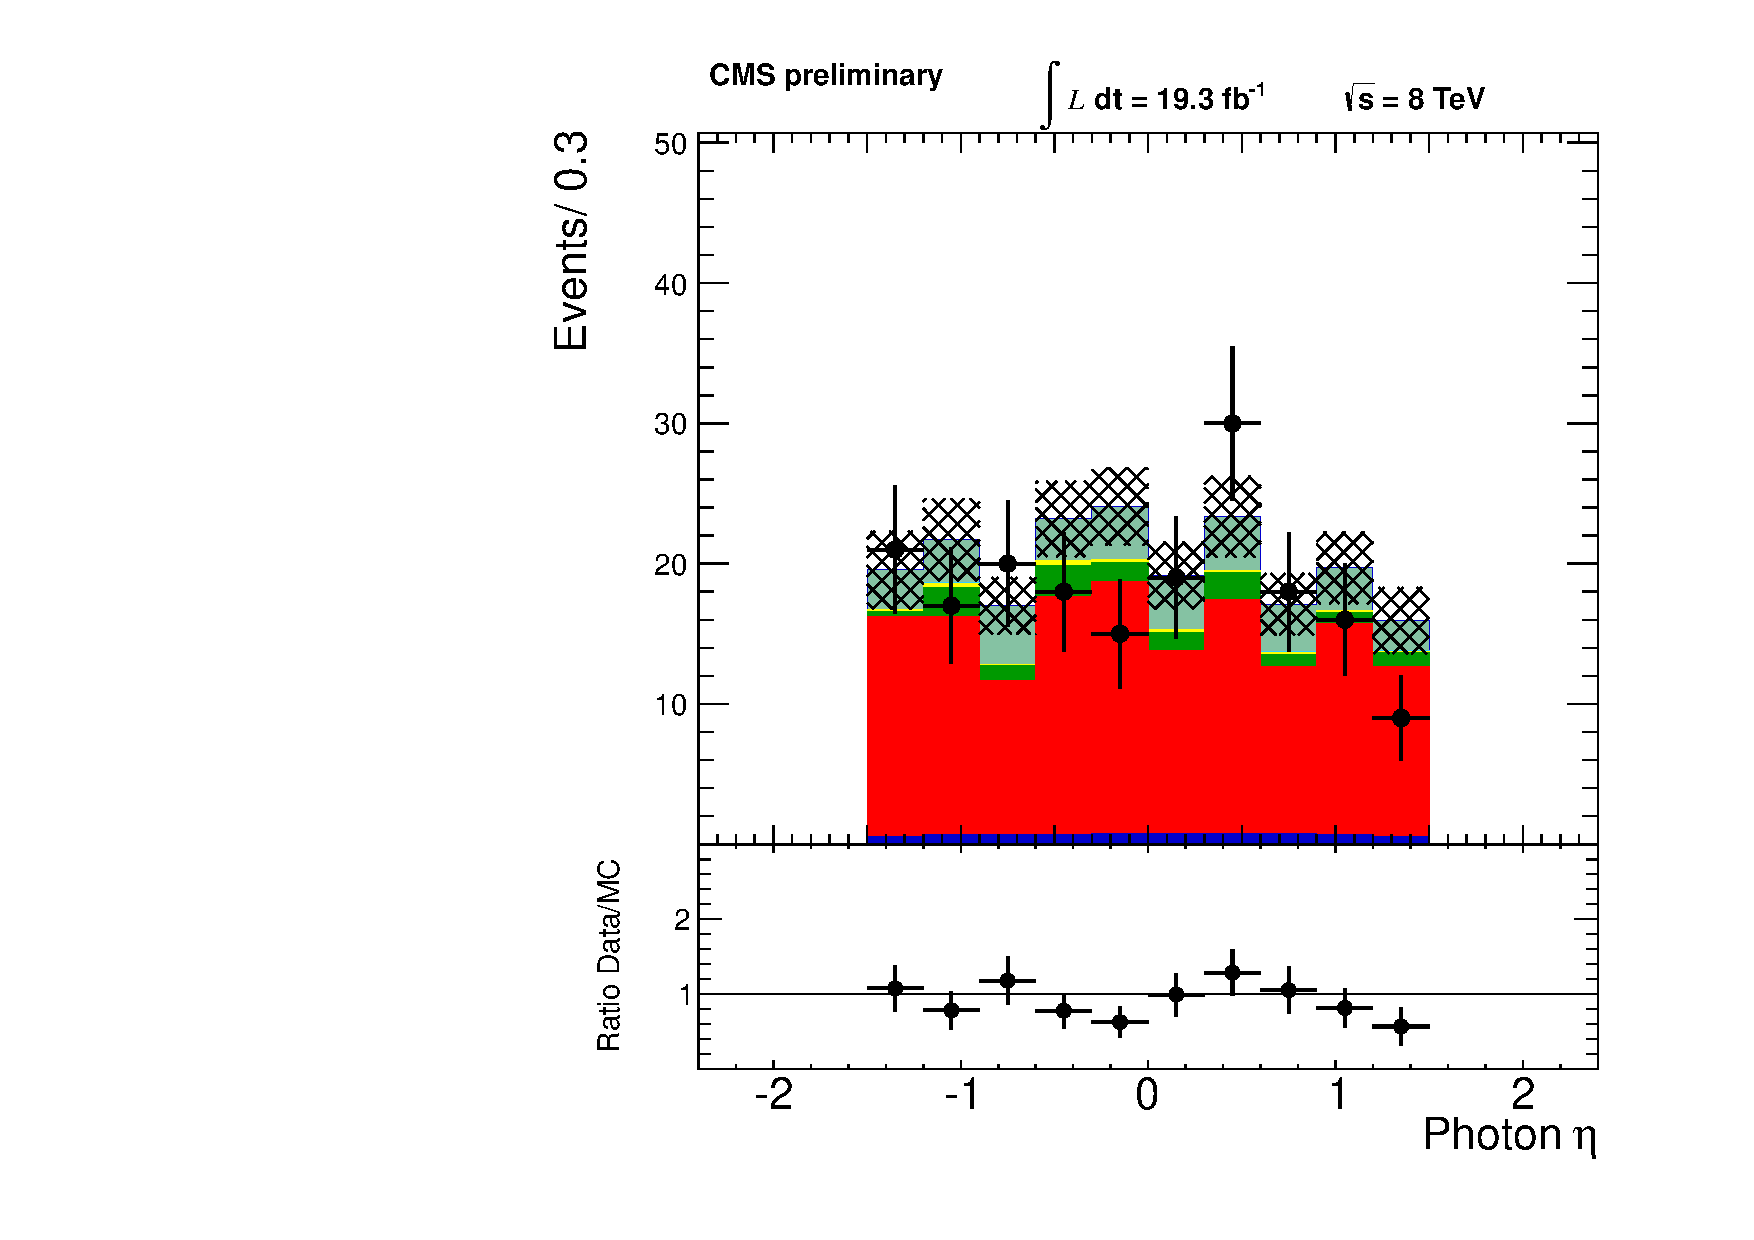
\includegraphics[width=.32\textwidth]{figs/mu_Photon_eta.pdf}
}
\subfigure[]{
   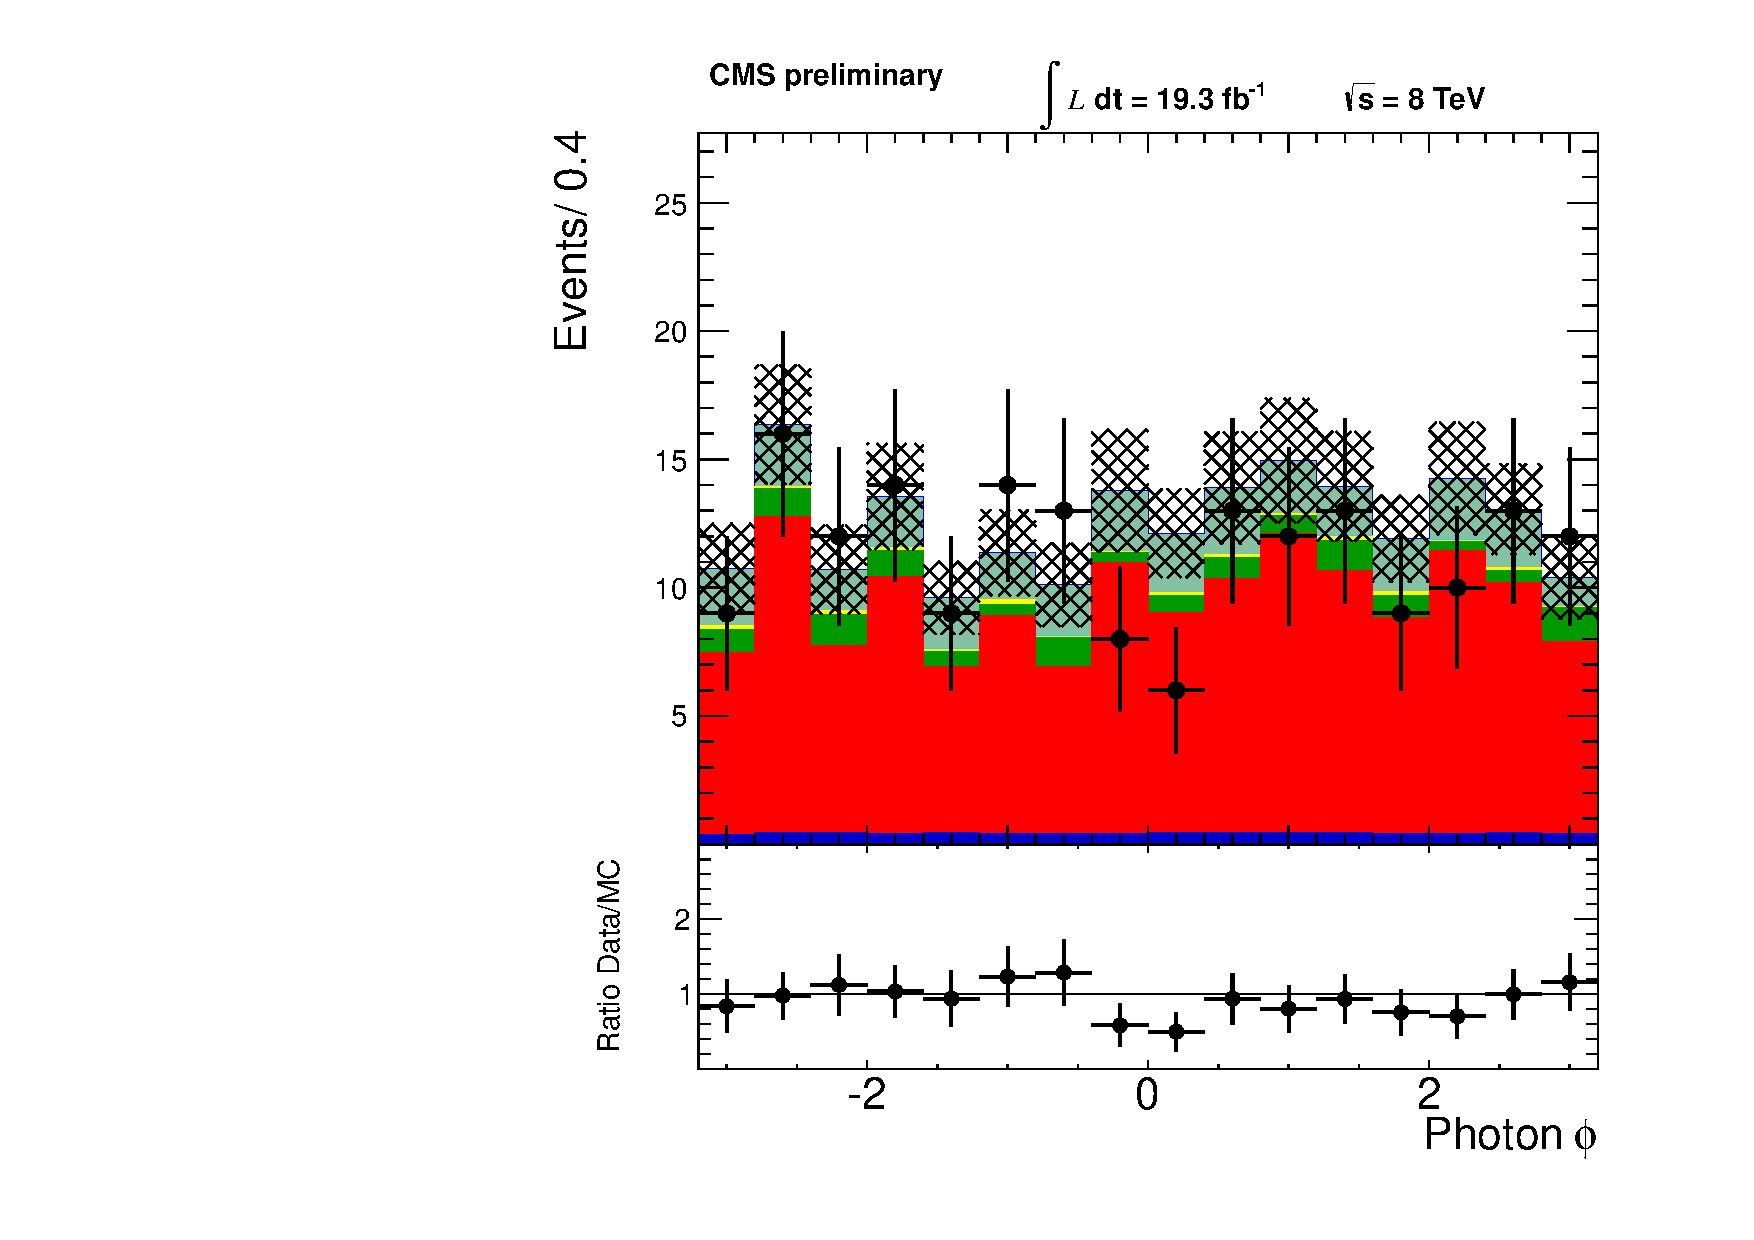
\includegraphics[width=.32\textwidth]{figs/mu_Photon_phi.pdf}
}\\
\subfigure[]{
   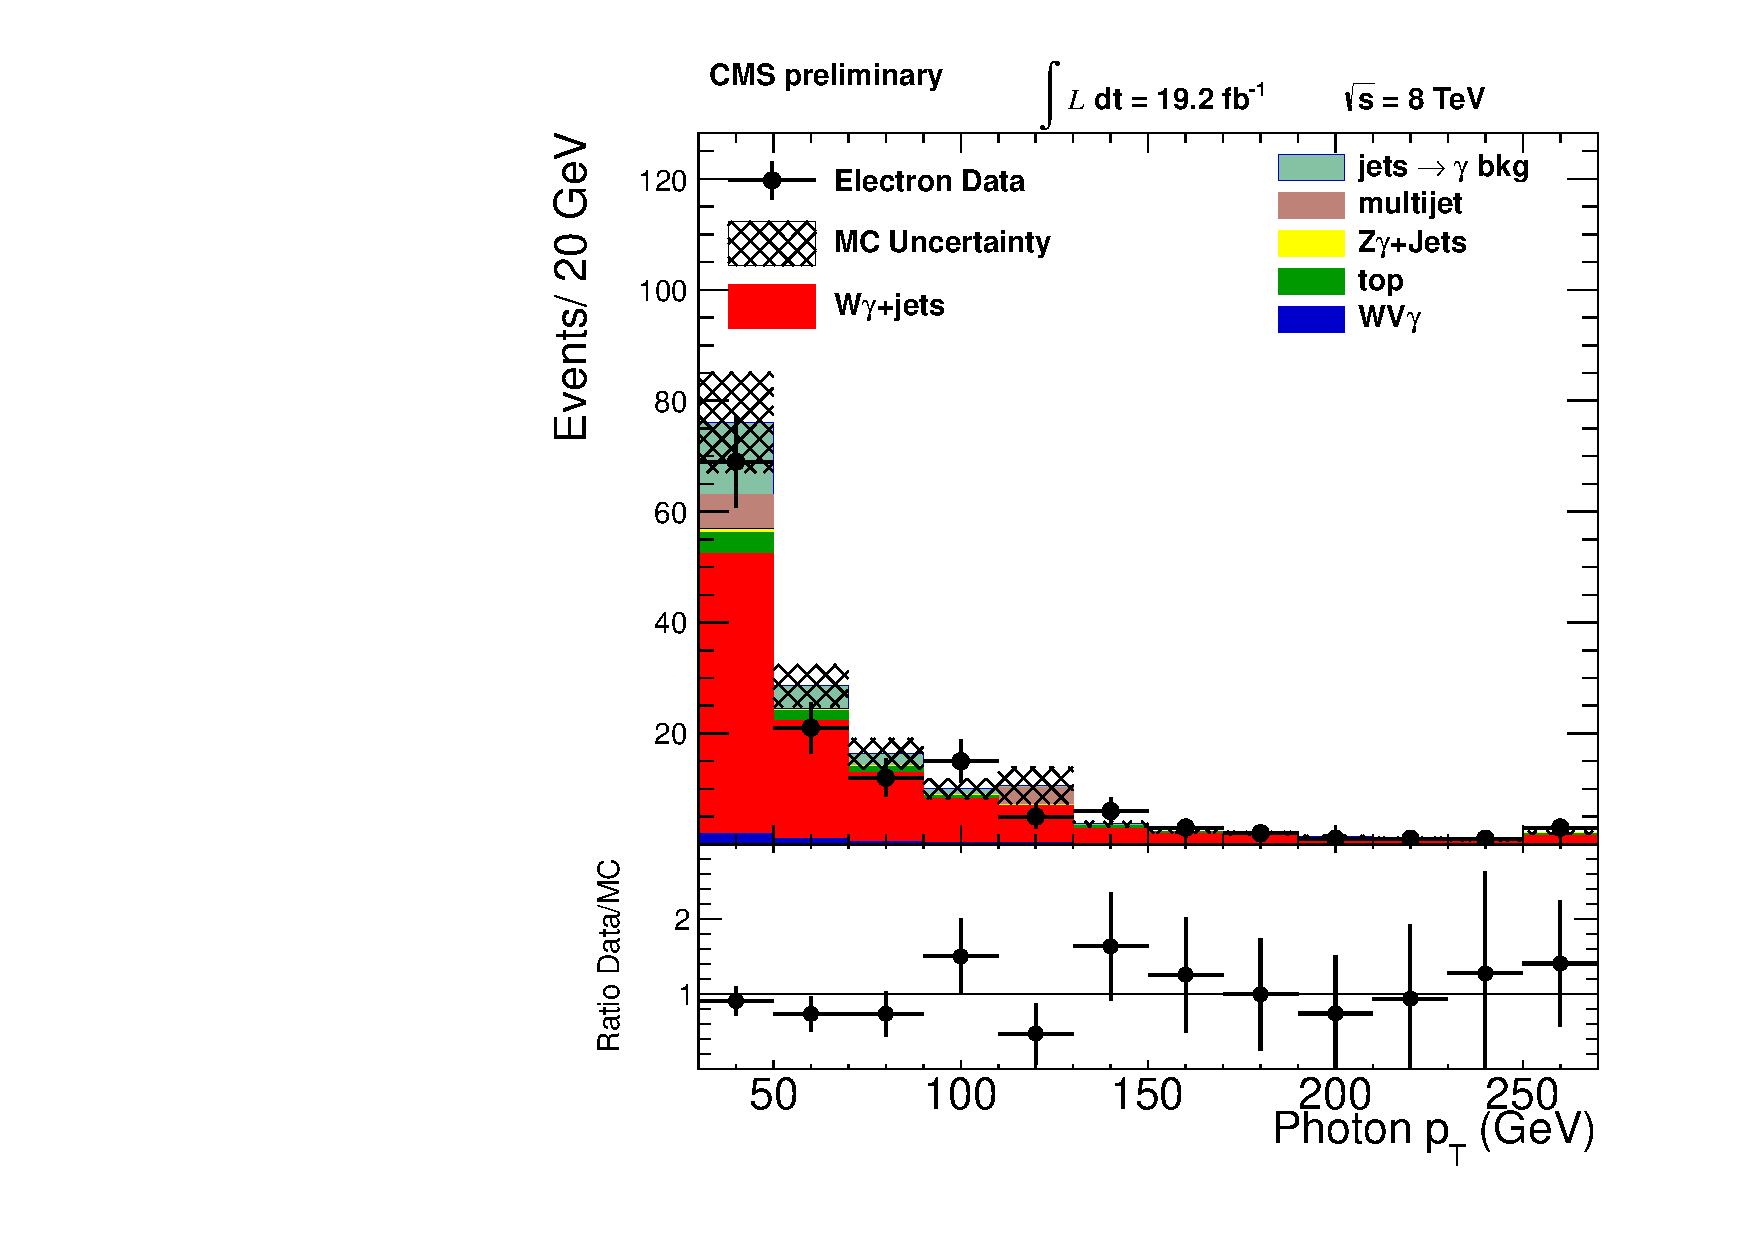
\includegraphics[width=.32\textwidth]{figs/el_Photon_pt.pdf}
}
\subfigure[]{
   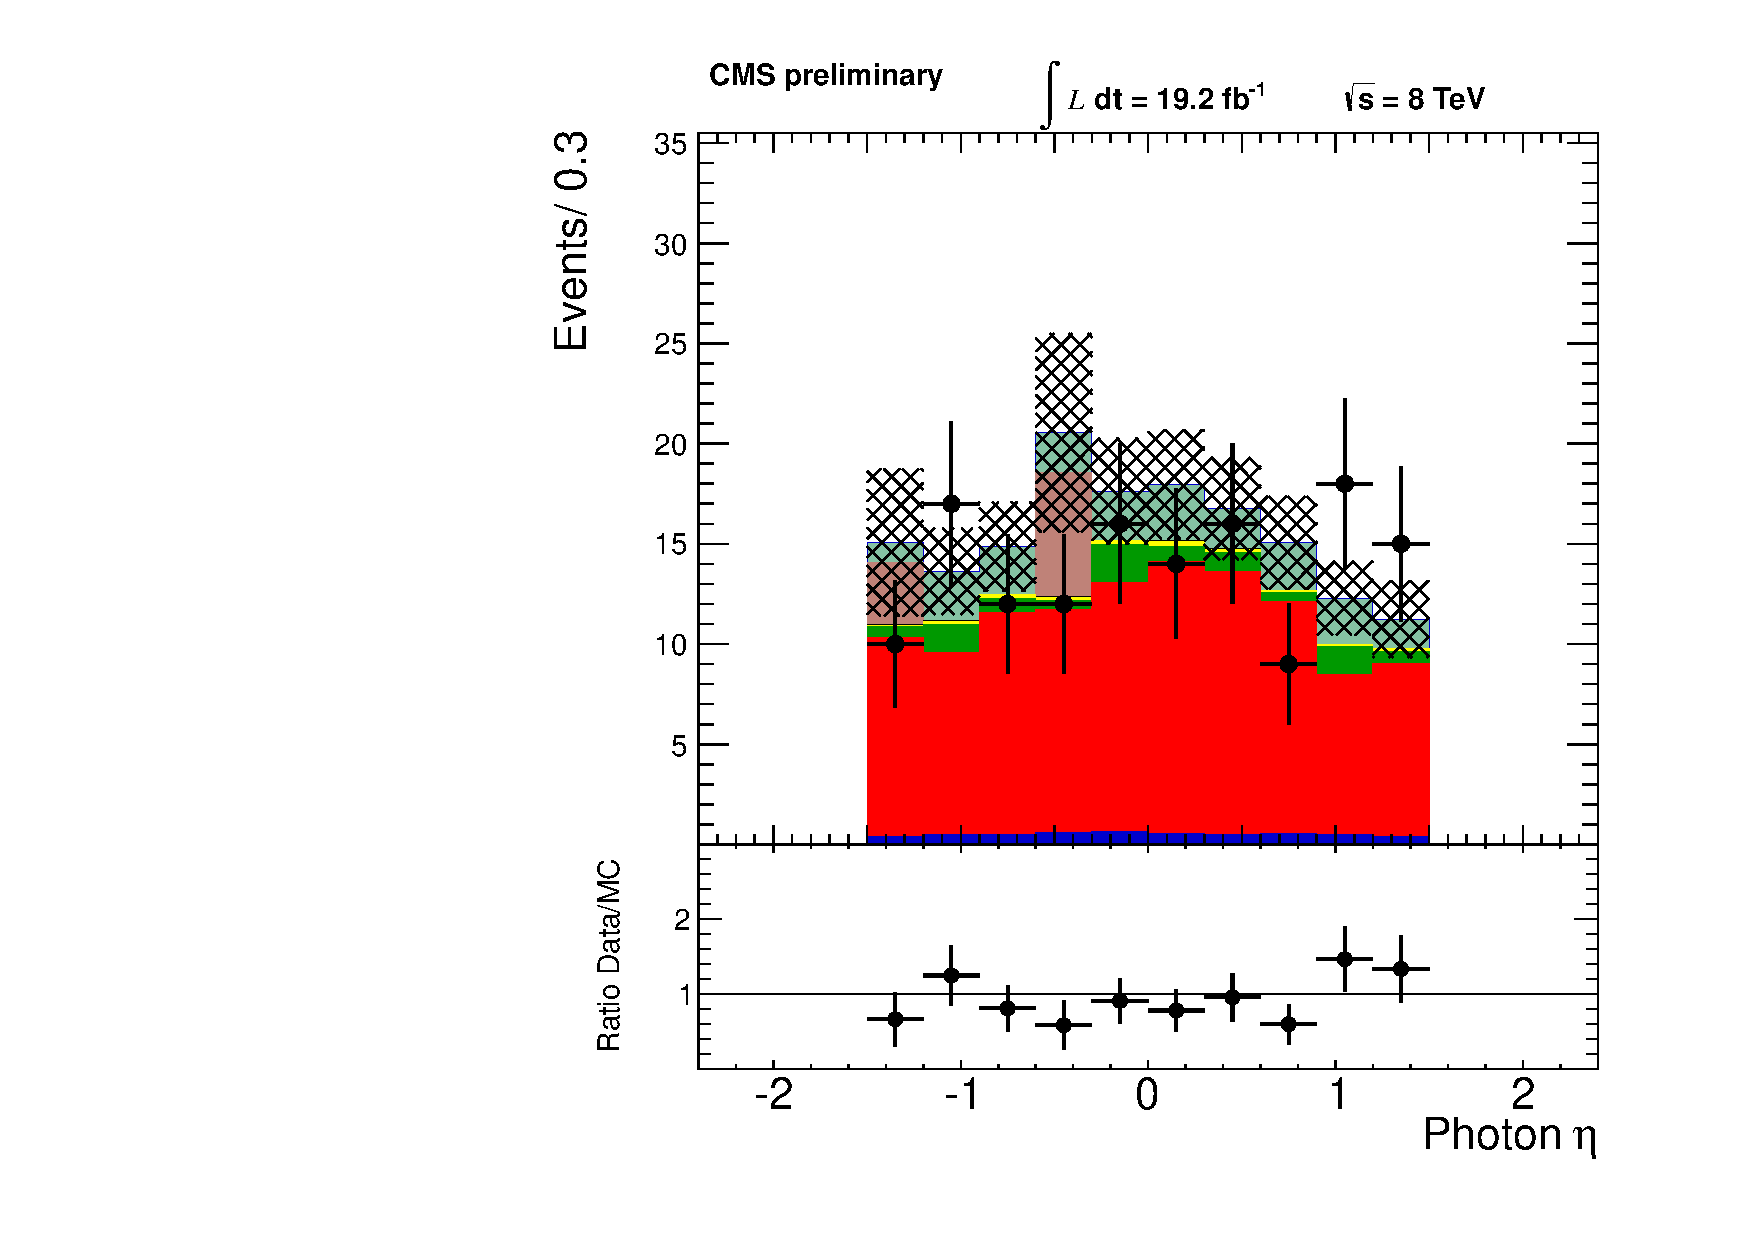
\includegraphics[width=.32\textwidth]{figs/el_Photon_eta.pdf}
}
\subfigure[]{
   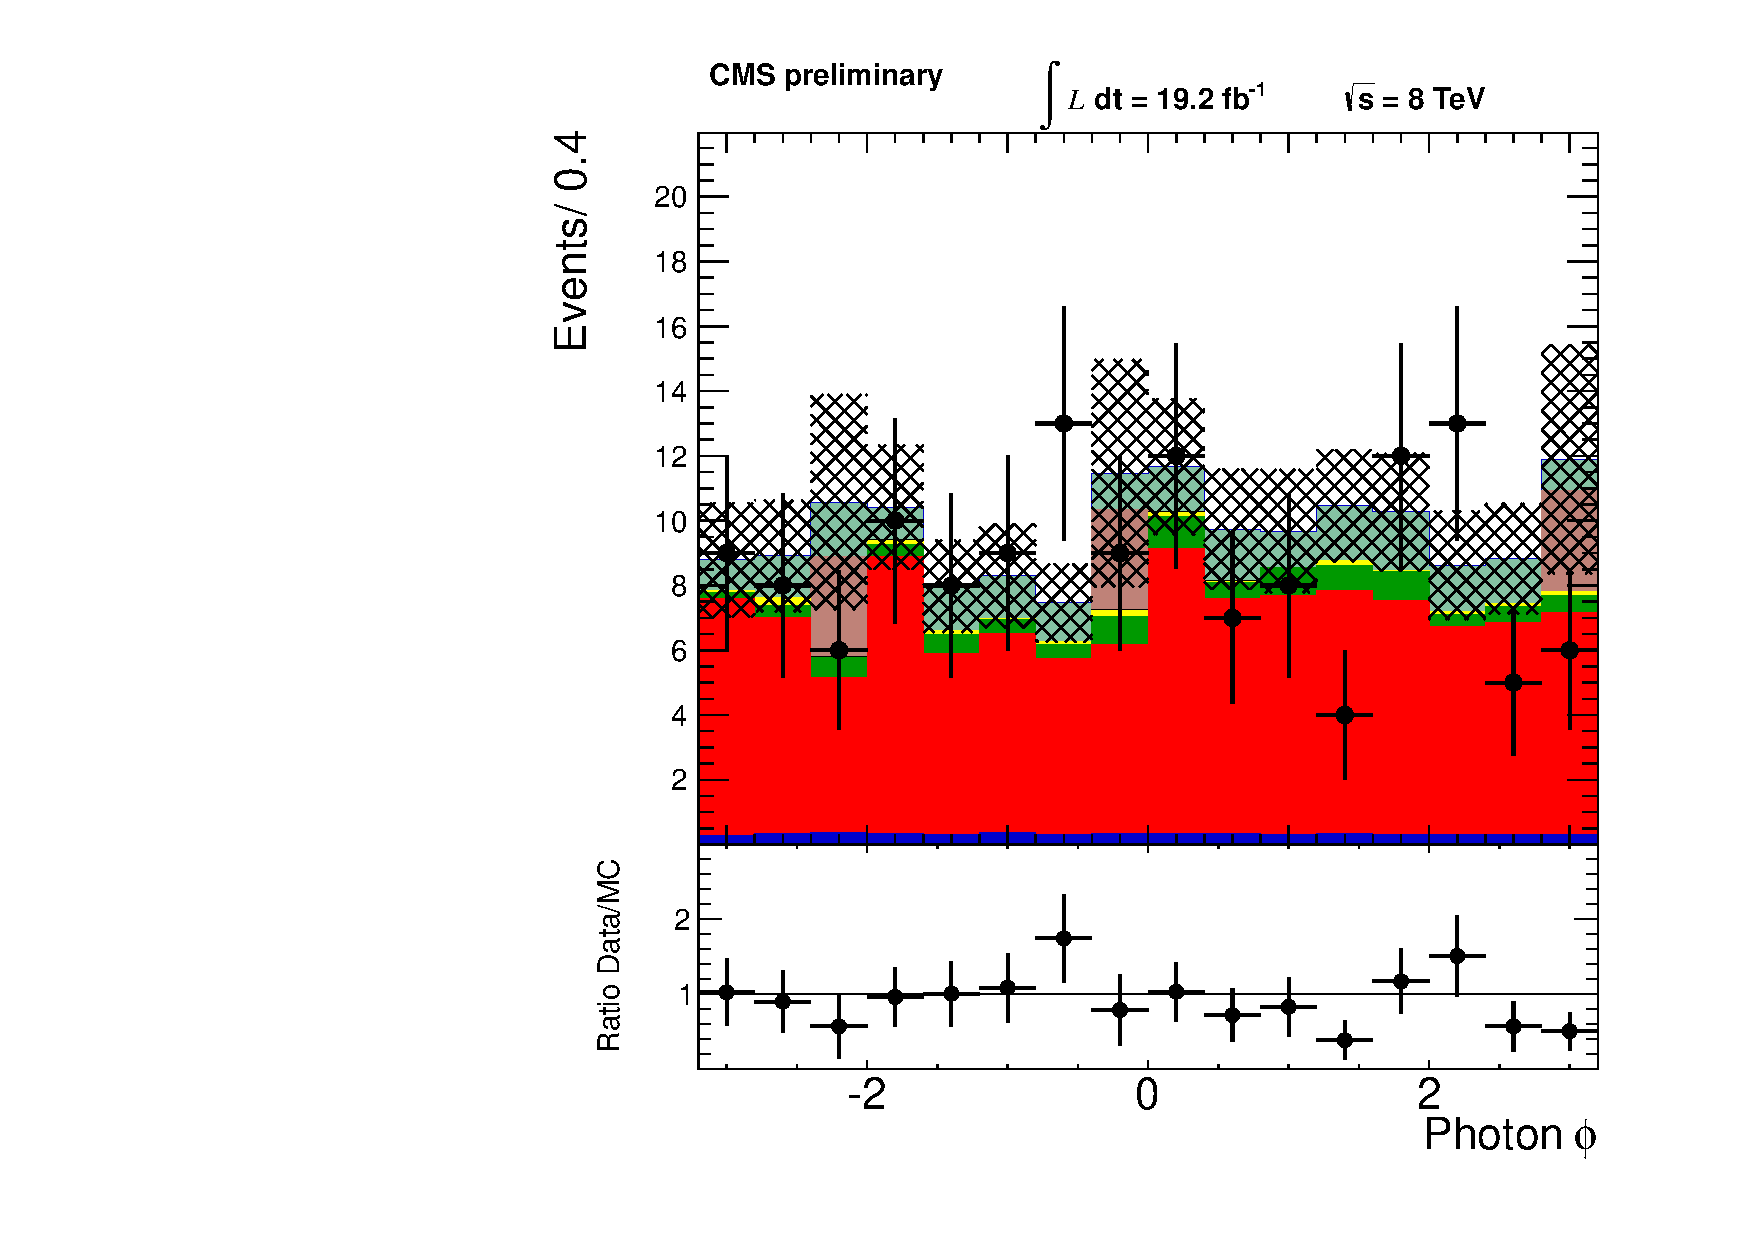
\includegraphics[width=.32\textwidth]{figs/el_Photon_phi.pdf}
}
\caption{Data and MC comparison plots for muon channel photon $p_{T}$ (a), $\eta$ (b), $\phi$ (c), and electron channel photon $p_{T}$ (d), $\eta$ (e), $\phi$ (f)}
\label{photonplots}
\end{center}
\end{figure}

\begin{figure}[b]
\begin{center}
\subfigure[]{
   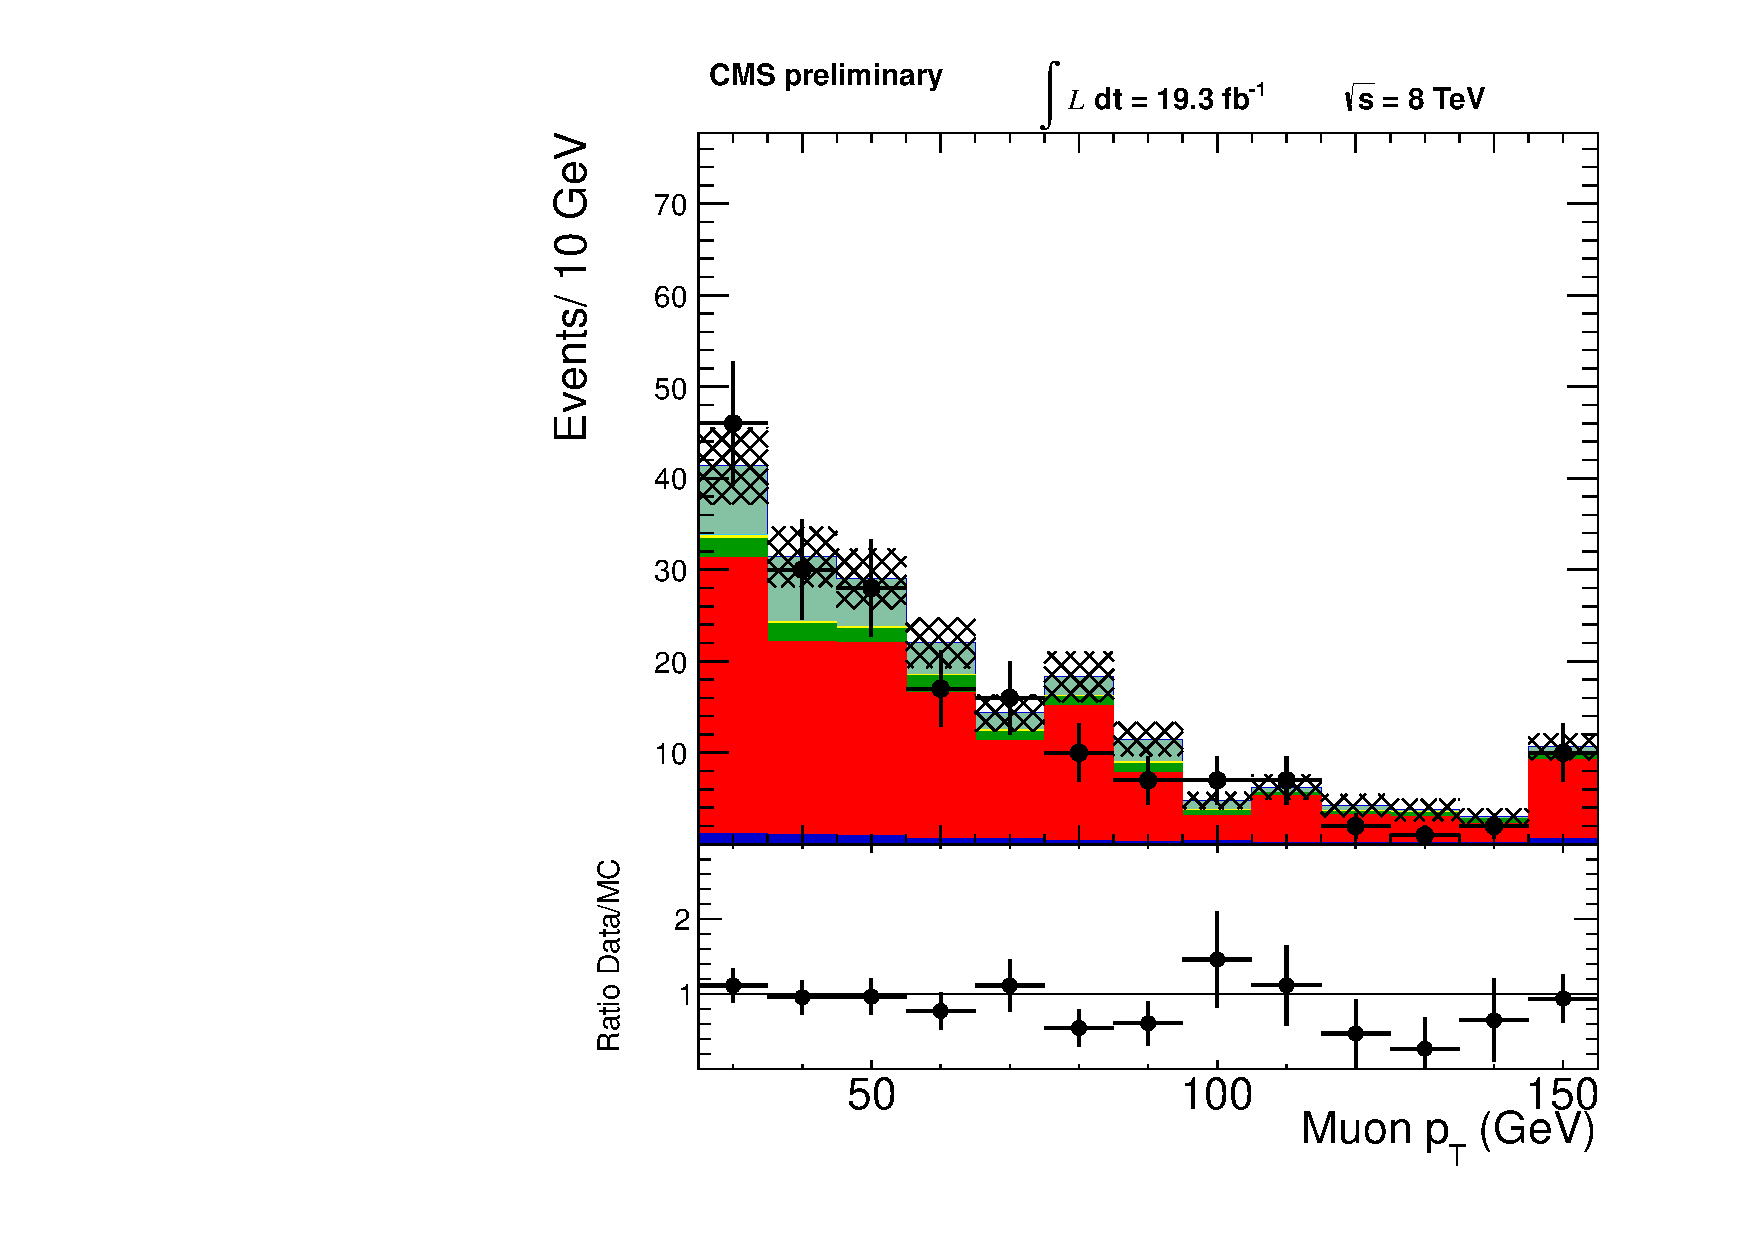
\includegraphics[width=.32\textwidth]{figs/mu_W_muon_pt.pdf}
}   
\subfigure[]{
   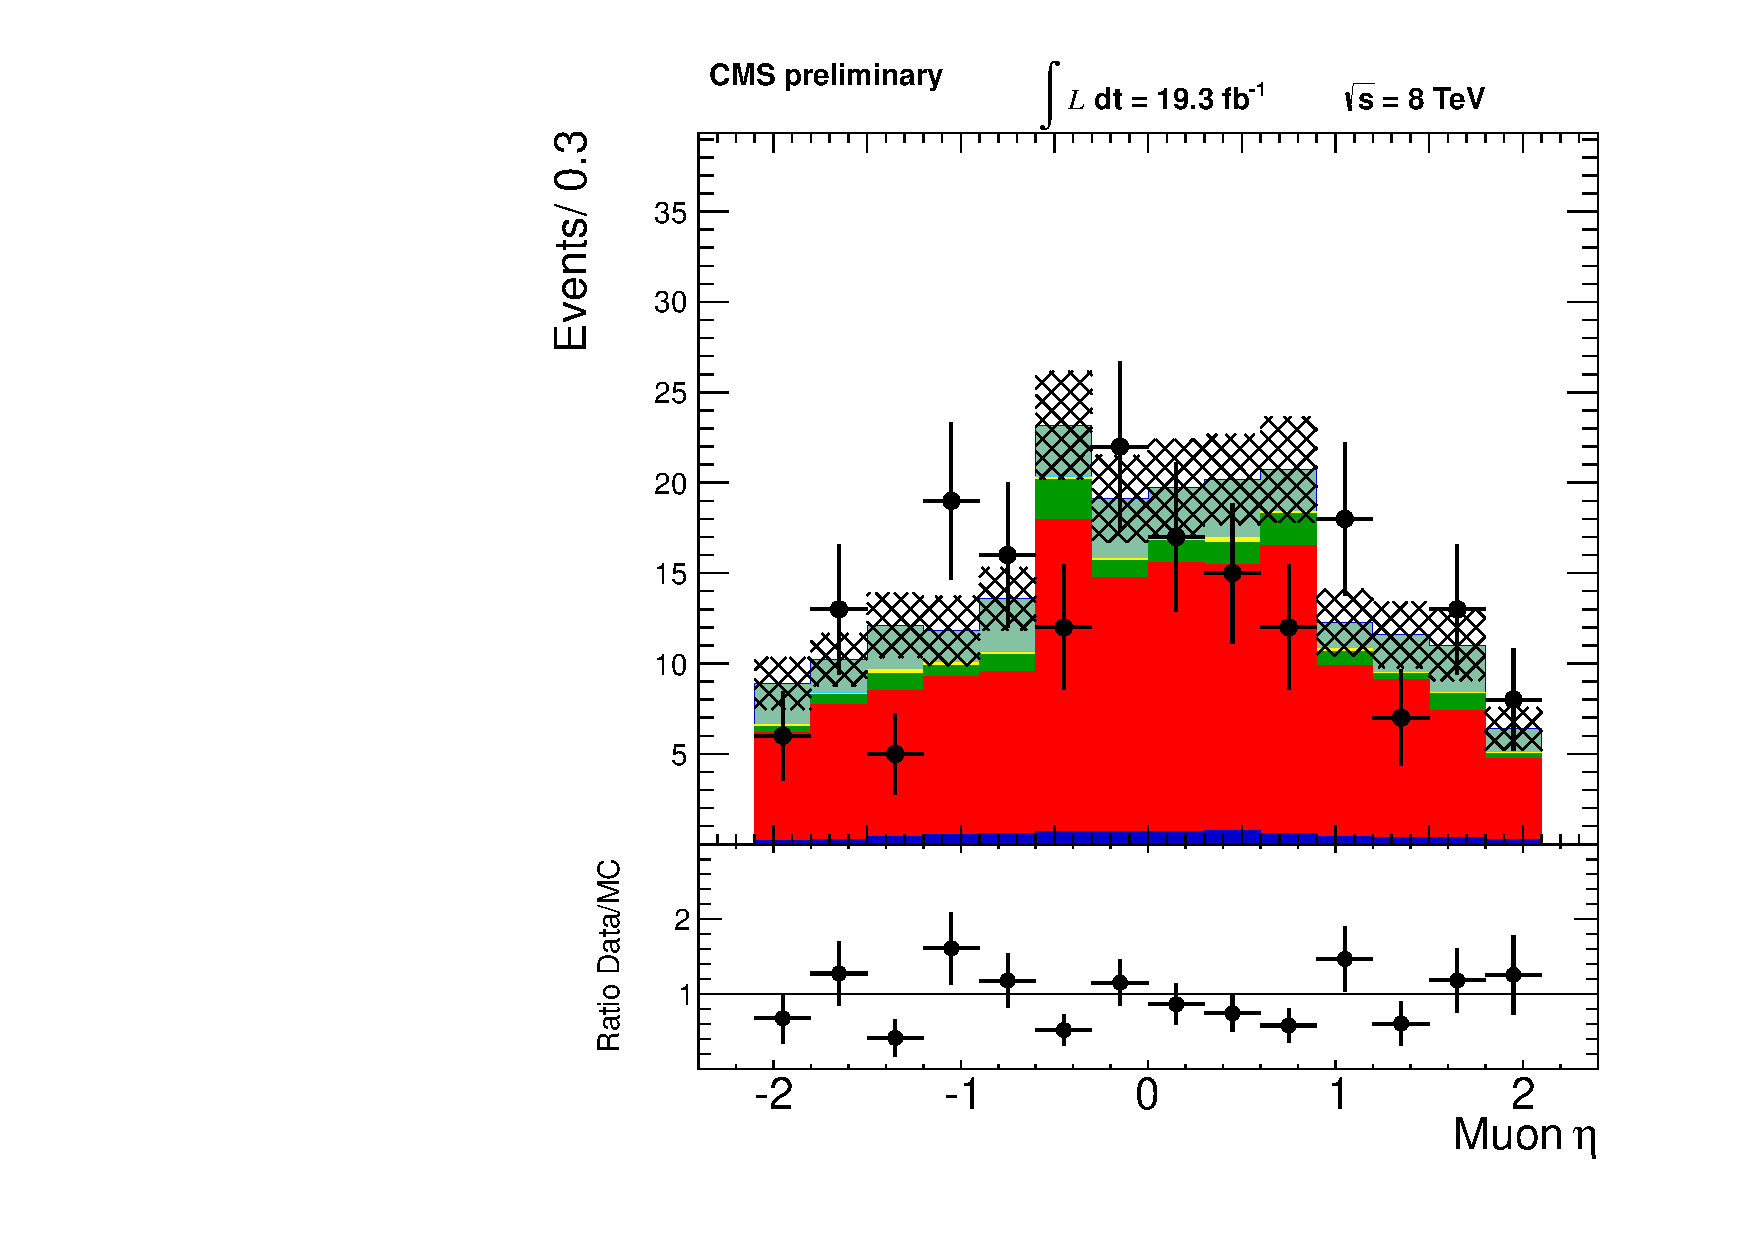
\includegraphics[width=.32\textwidth]{figs/mu_W_muon_eta.pdf}
}   
\subfigure[]{
   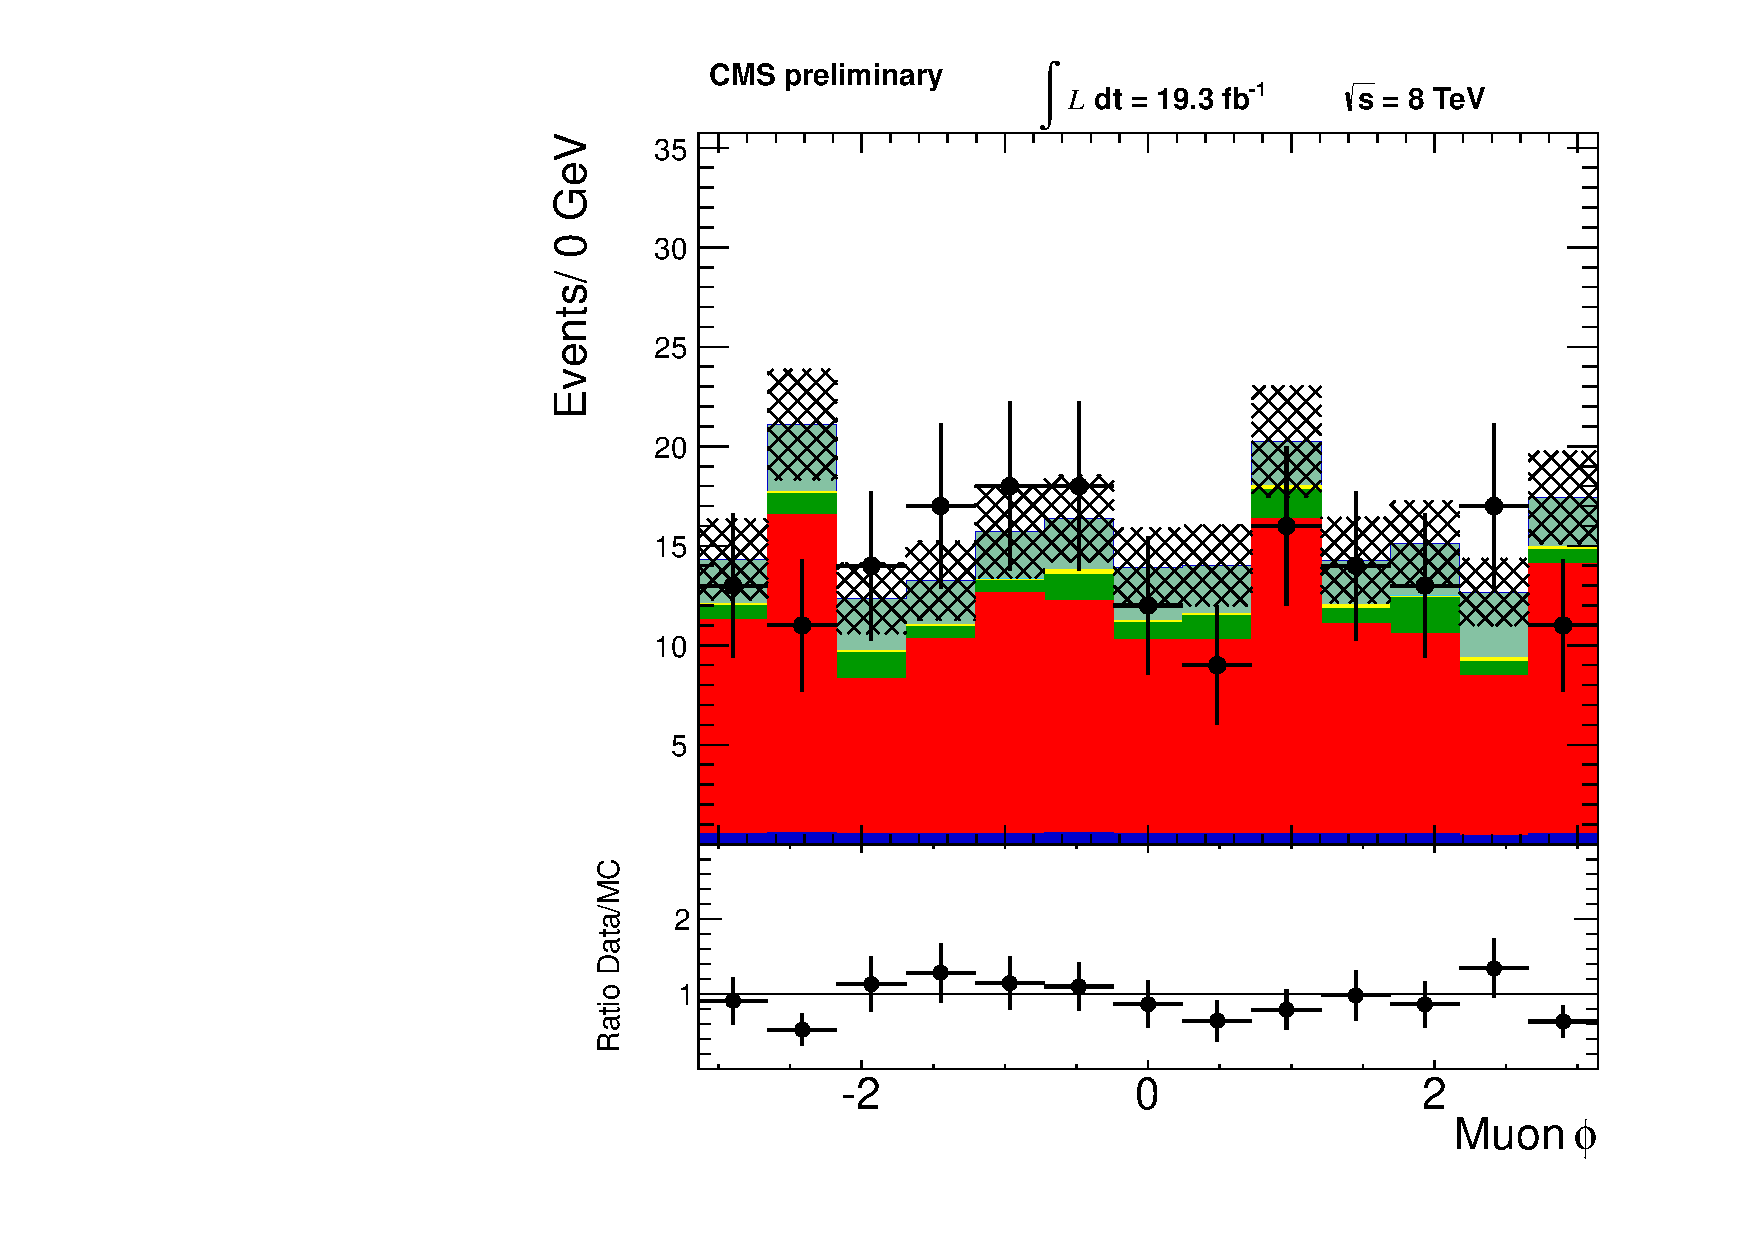
\includegraphics[width=.32\textwidth]{figs/mu_W_muon_phi.pdf}
}
\caption{Data and MC comparison plots for muon $p_{T}$ (a), $\eta$ (b), $\phi$ (c)}
\label{muonplots}
\end{center}
\end{figure}

\begin{figure}[b]
\begin{center}
\subfigure[]{
   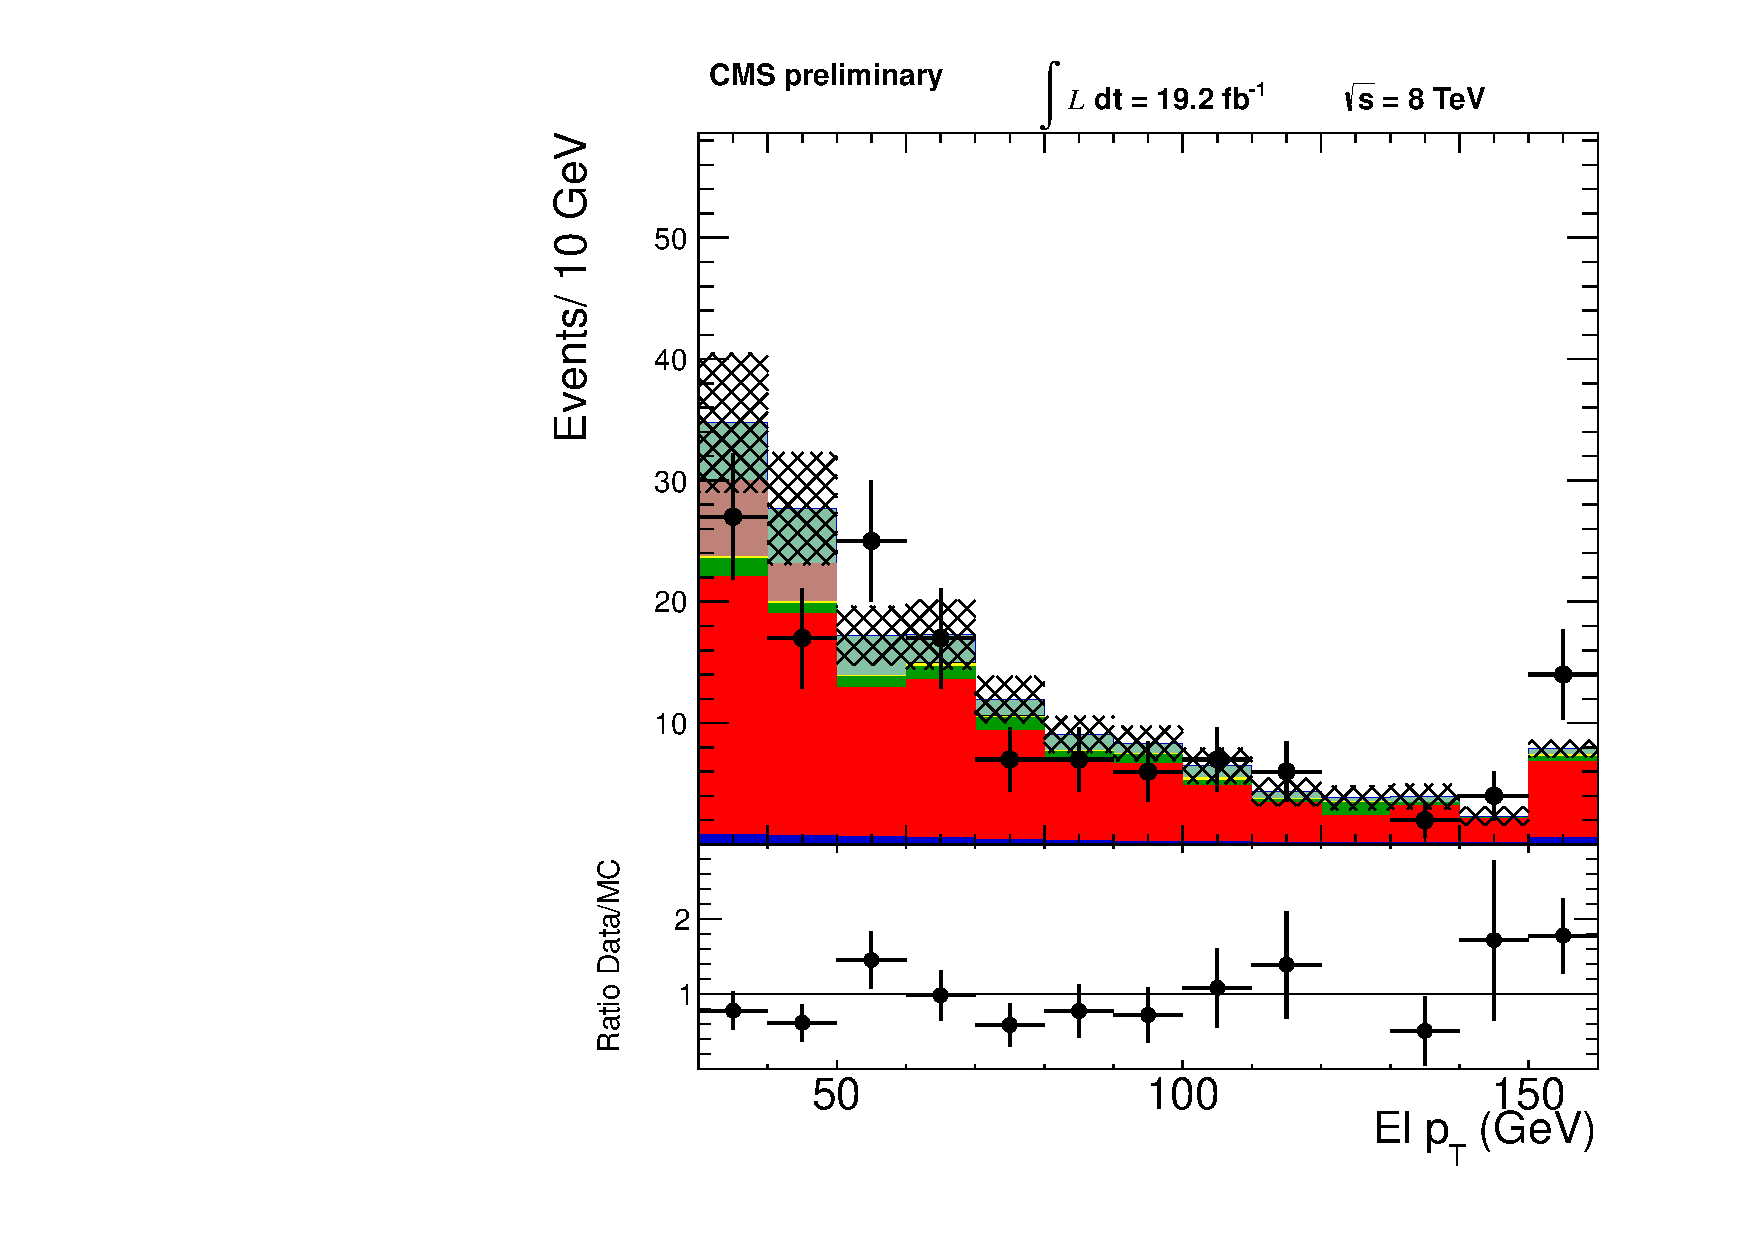
\includegraphics[width=.32\textwidth]{figs/el_W_electron_pt.pdf}
}   
\subfigure[]{
   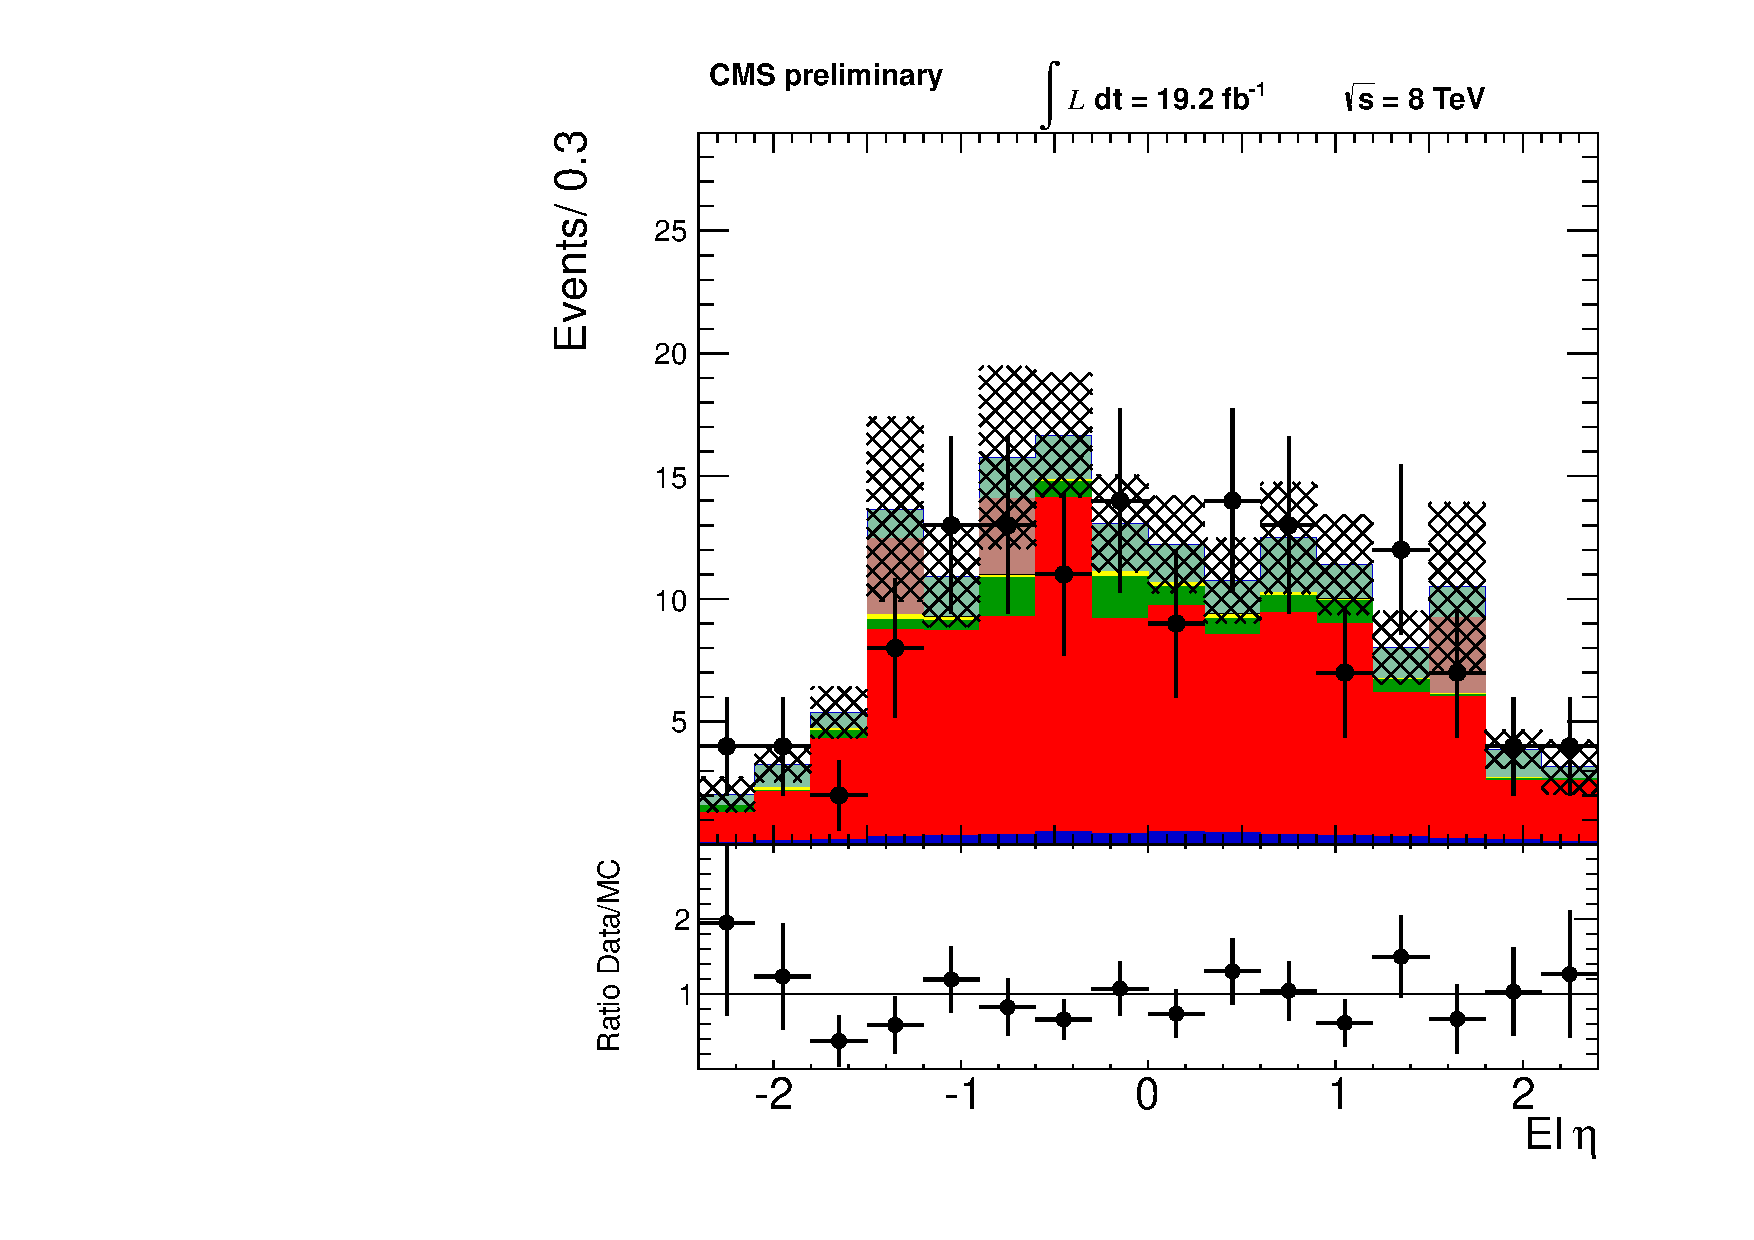
\includegraphics[width=.32\textwidth]{figs/el_W_electron_eta.pdf}
}   
\subfigure[]{
   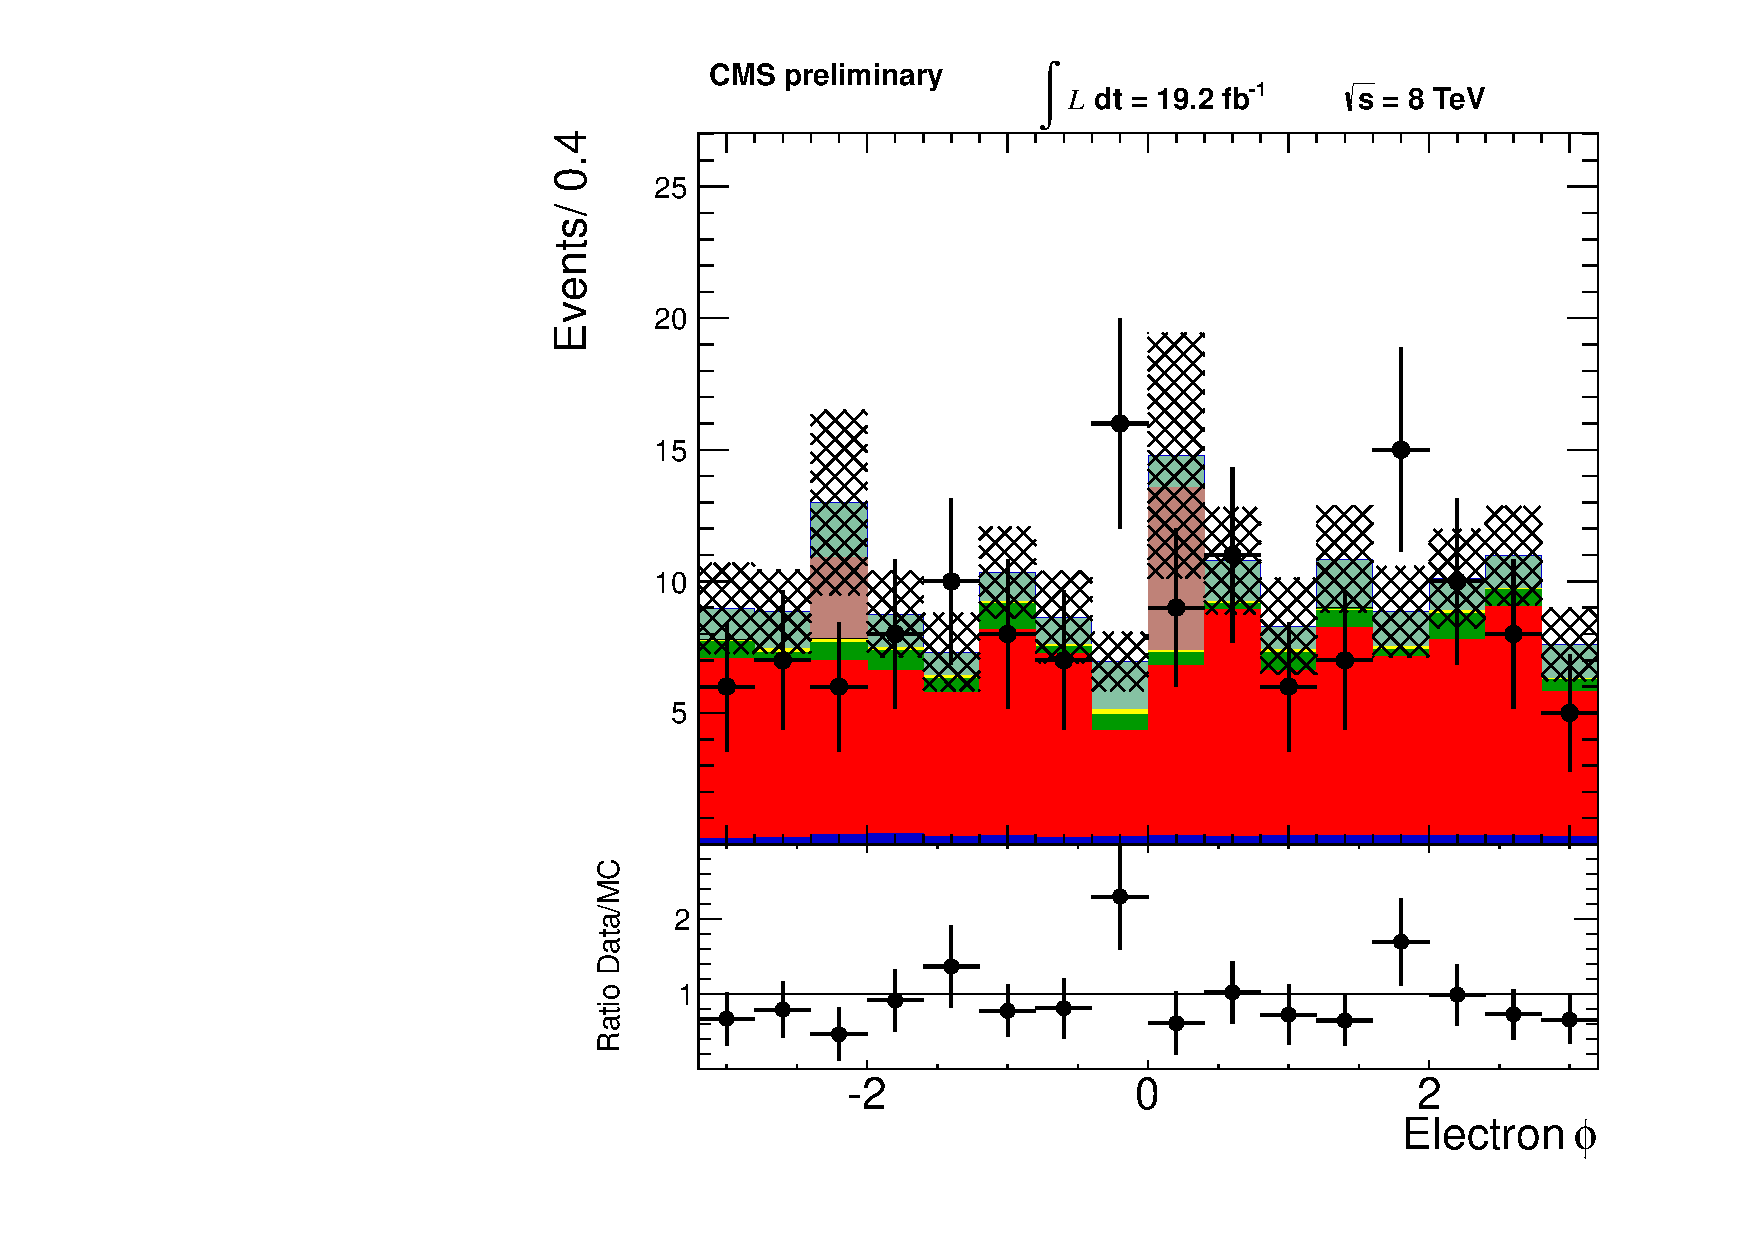
\includegraphics[width=.32\textwidth]{figs/el_W_electron_phi.pdf}
}
\caption{Data and MC comparison plots for electron $p_{T}$ (a), $\eta$ (b), $\phi$ (c)}
\label{elecplots}
\end{center}
\end{figure}

\begin{figure}[b]
\begin{center}
\subfigure[]{
   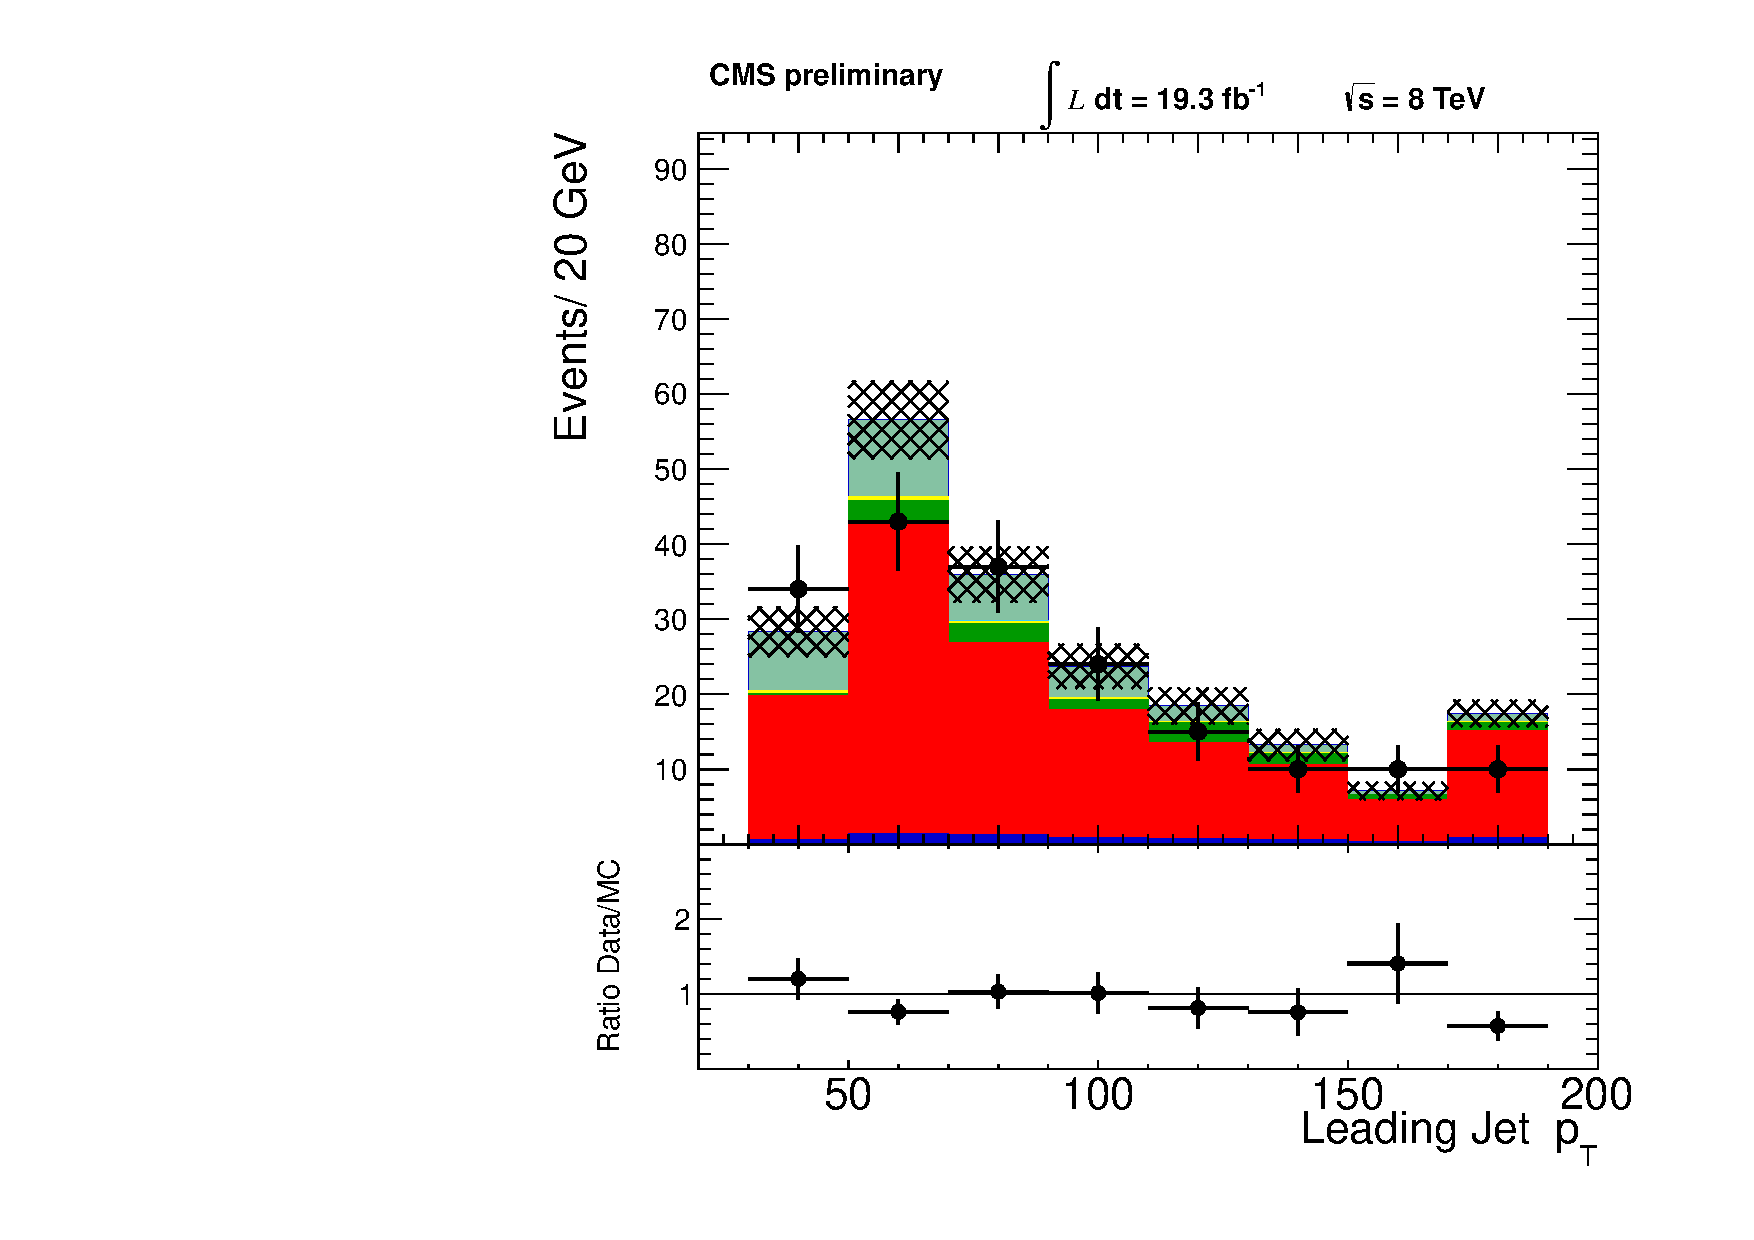
\includegraphics[width=.32\textwidth]{figs/mu_jetld_pt.pdf}
}   
\subfigure[]{
   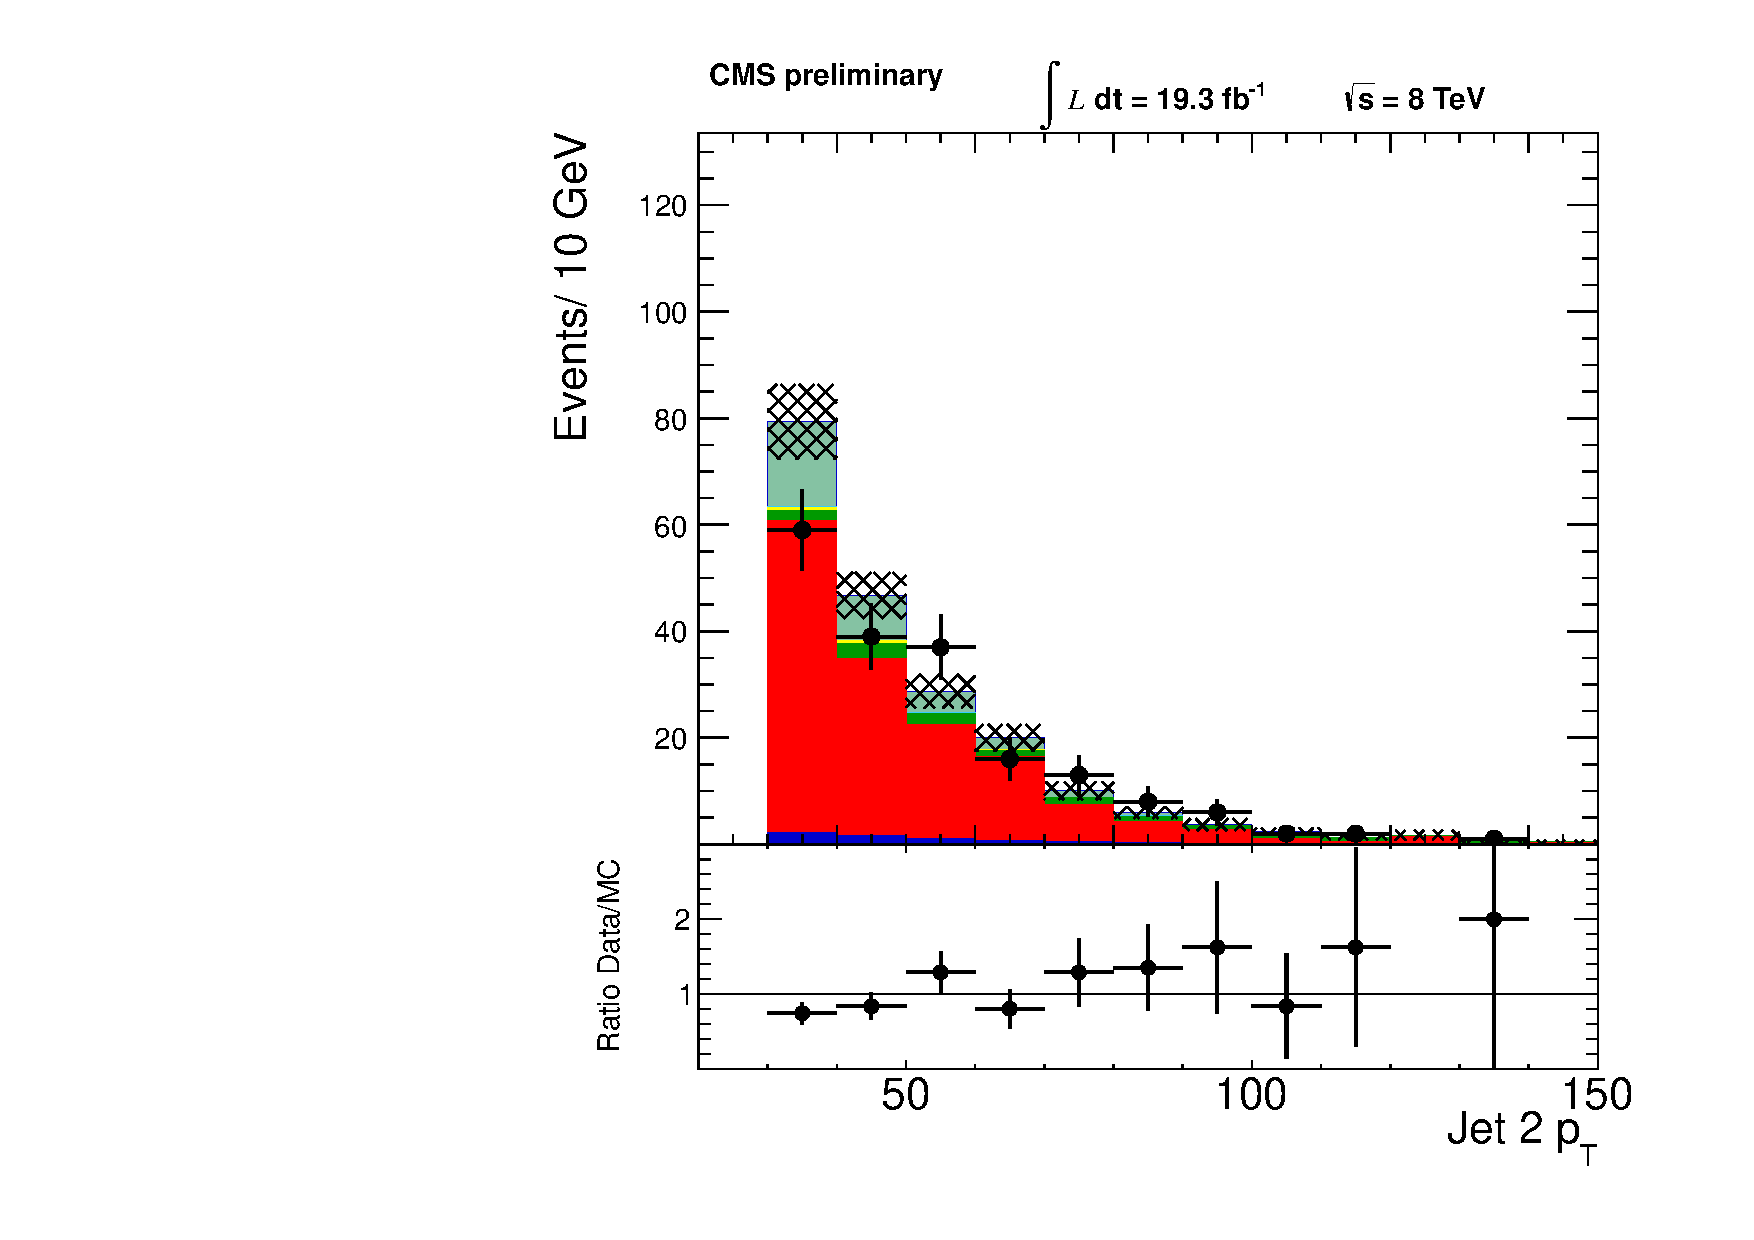
\includegraphics[width=.32\textwidth]{figs/mu_jetnt_pt.pdf}
}   
\subfigure[]{
   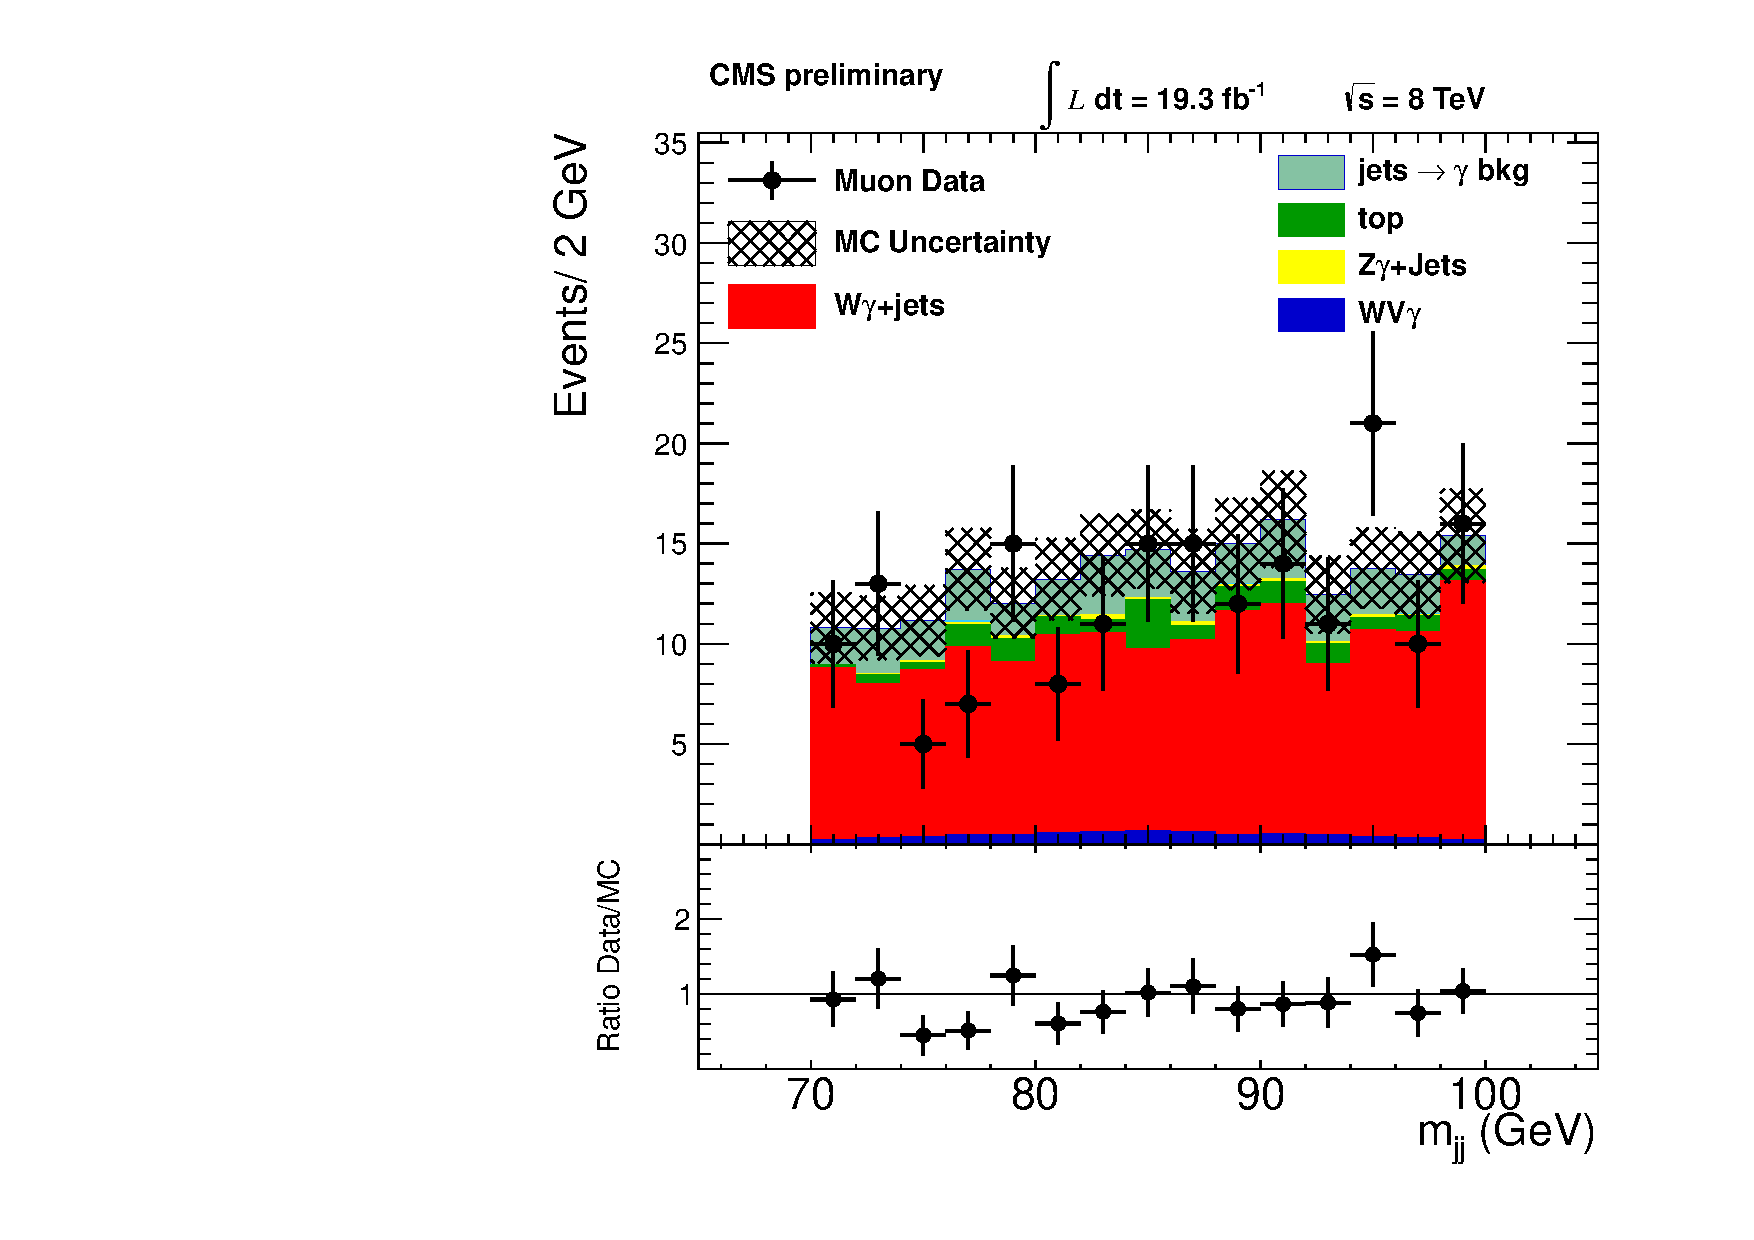
\includegraphics[width=.32\textwidth]{figs/mu_mjj.pdf}
}   \\
\subfigure[]{
   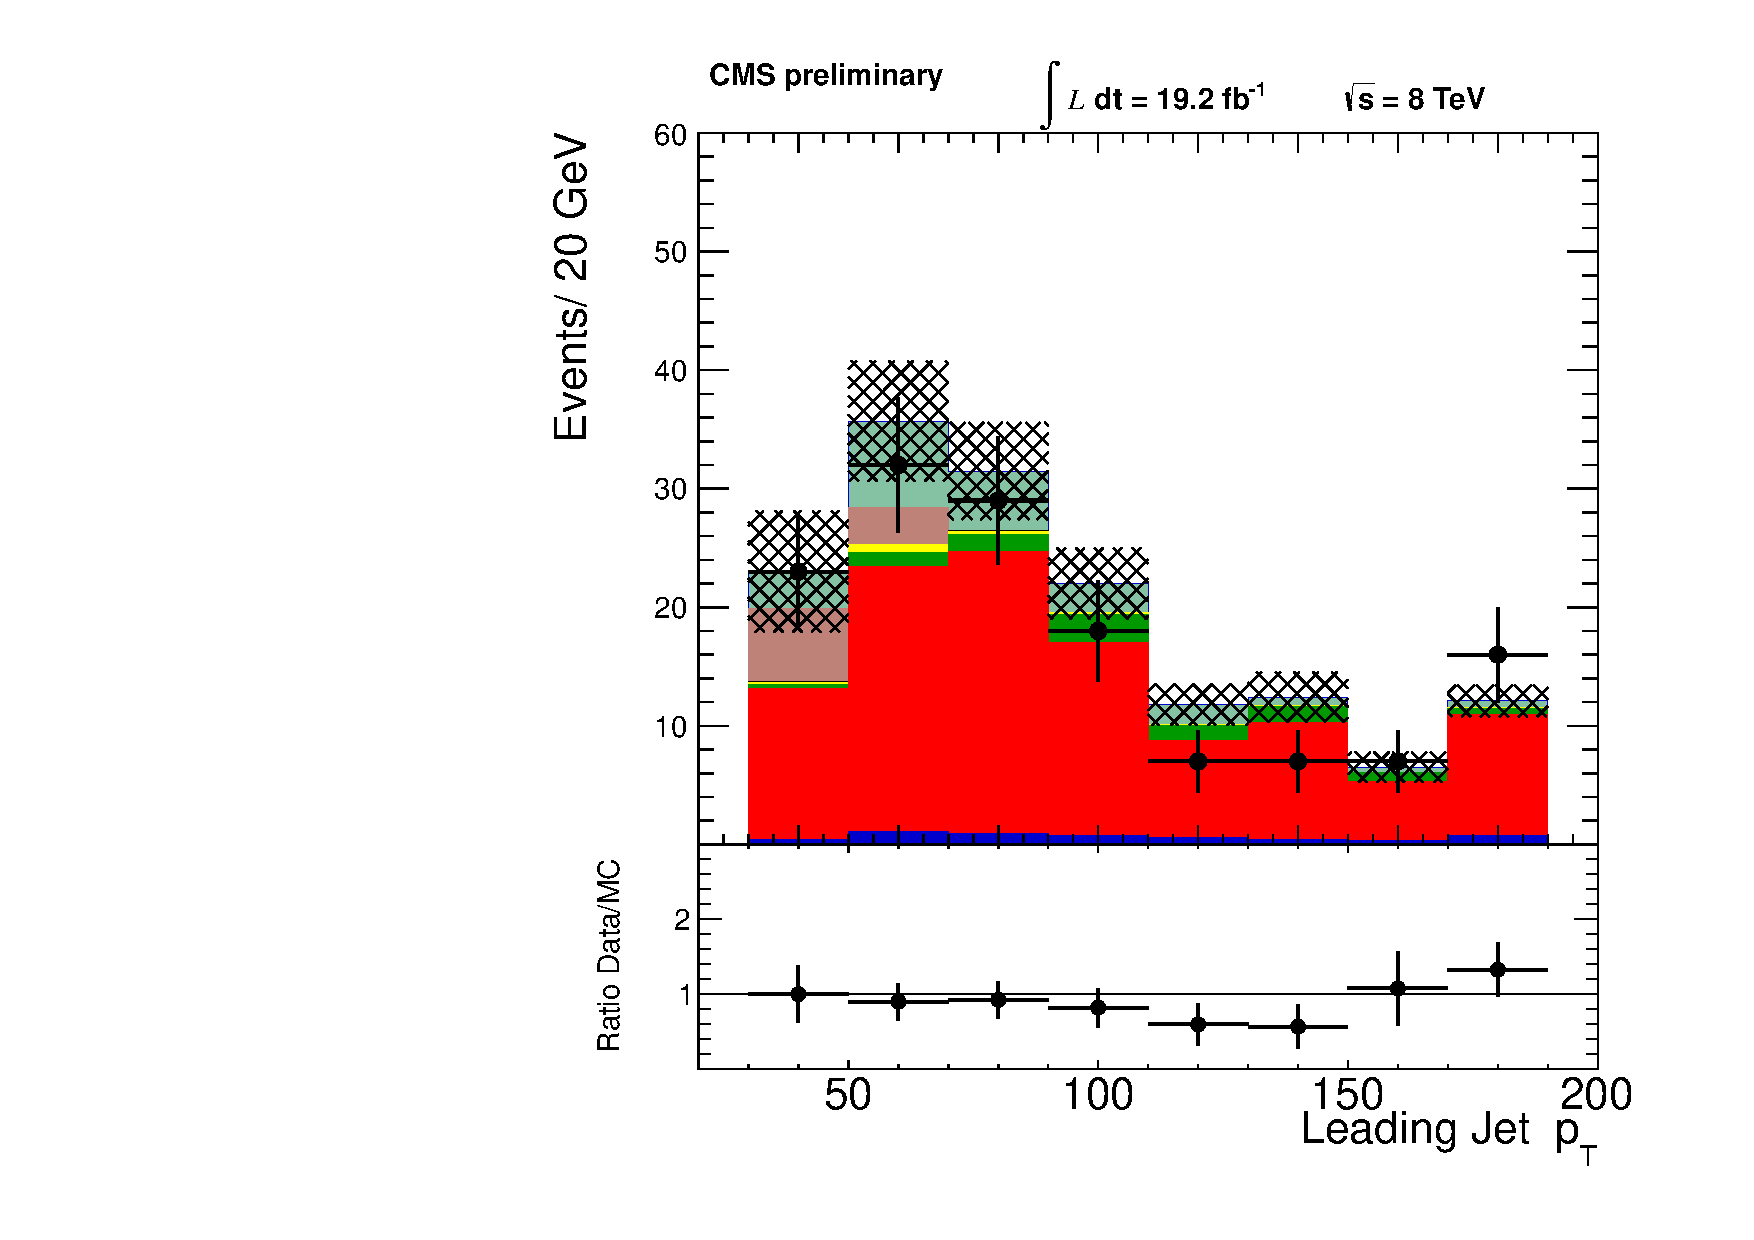
\includegraphics[width=.32\textwidth]{figs/el_jetld_pt.pdf}
}   
\subfigure[]{
   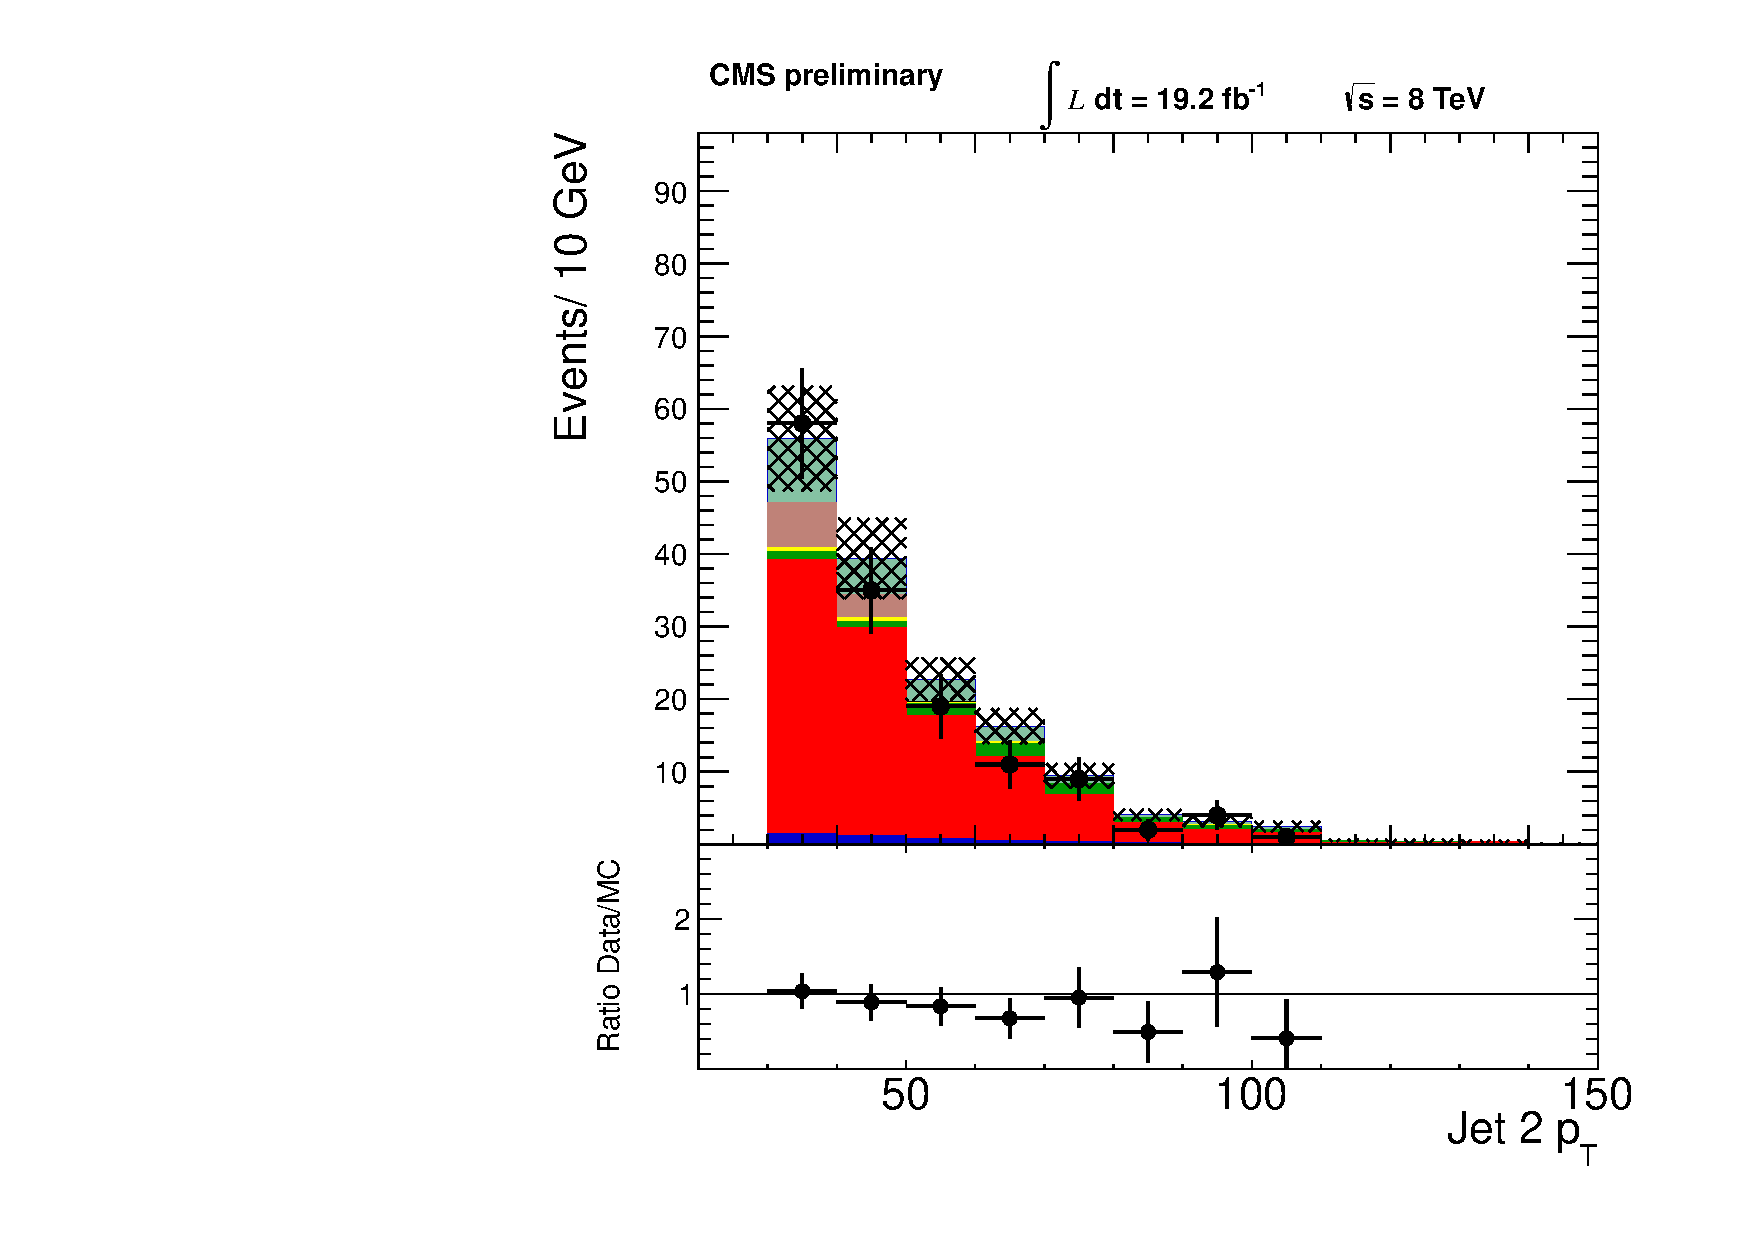
\includegraphics[width=.32\textwidth]{figs/el_jetnt_pt.pdf}
}   
\subfigure[]{
   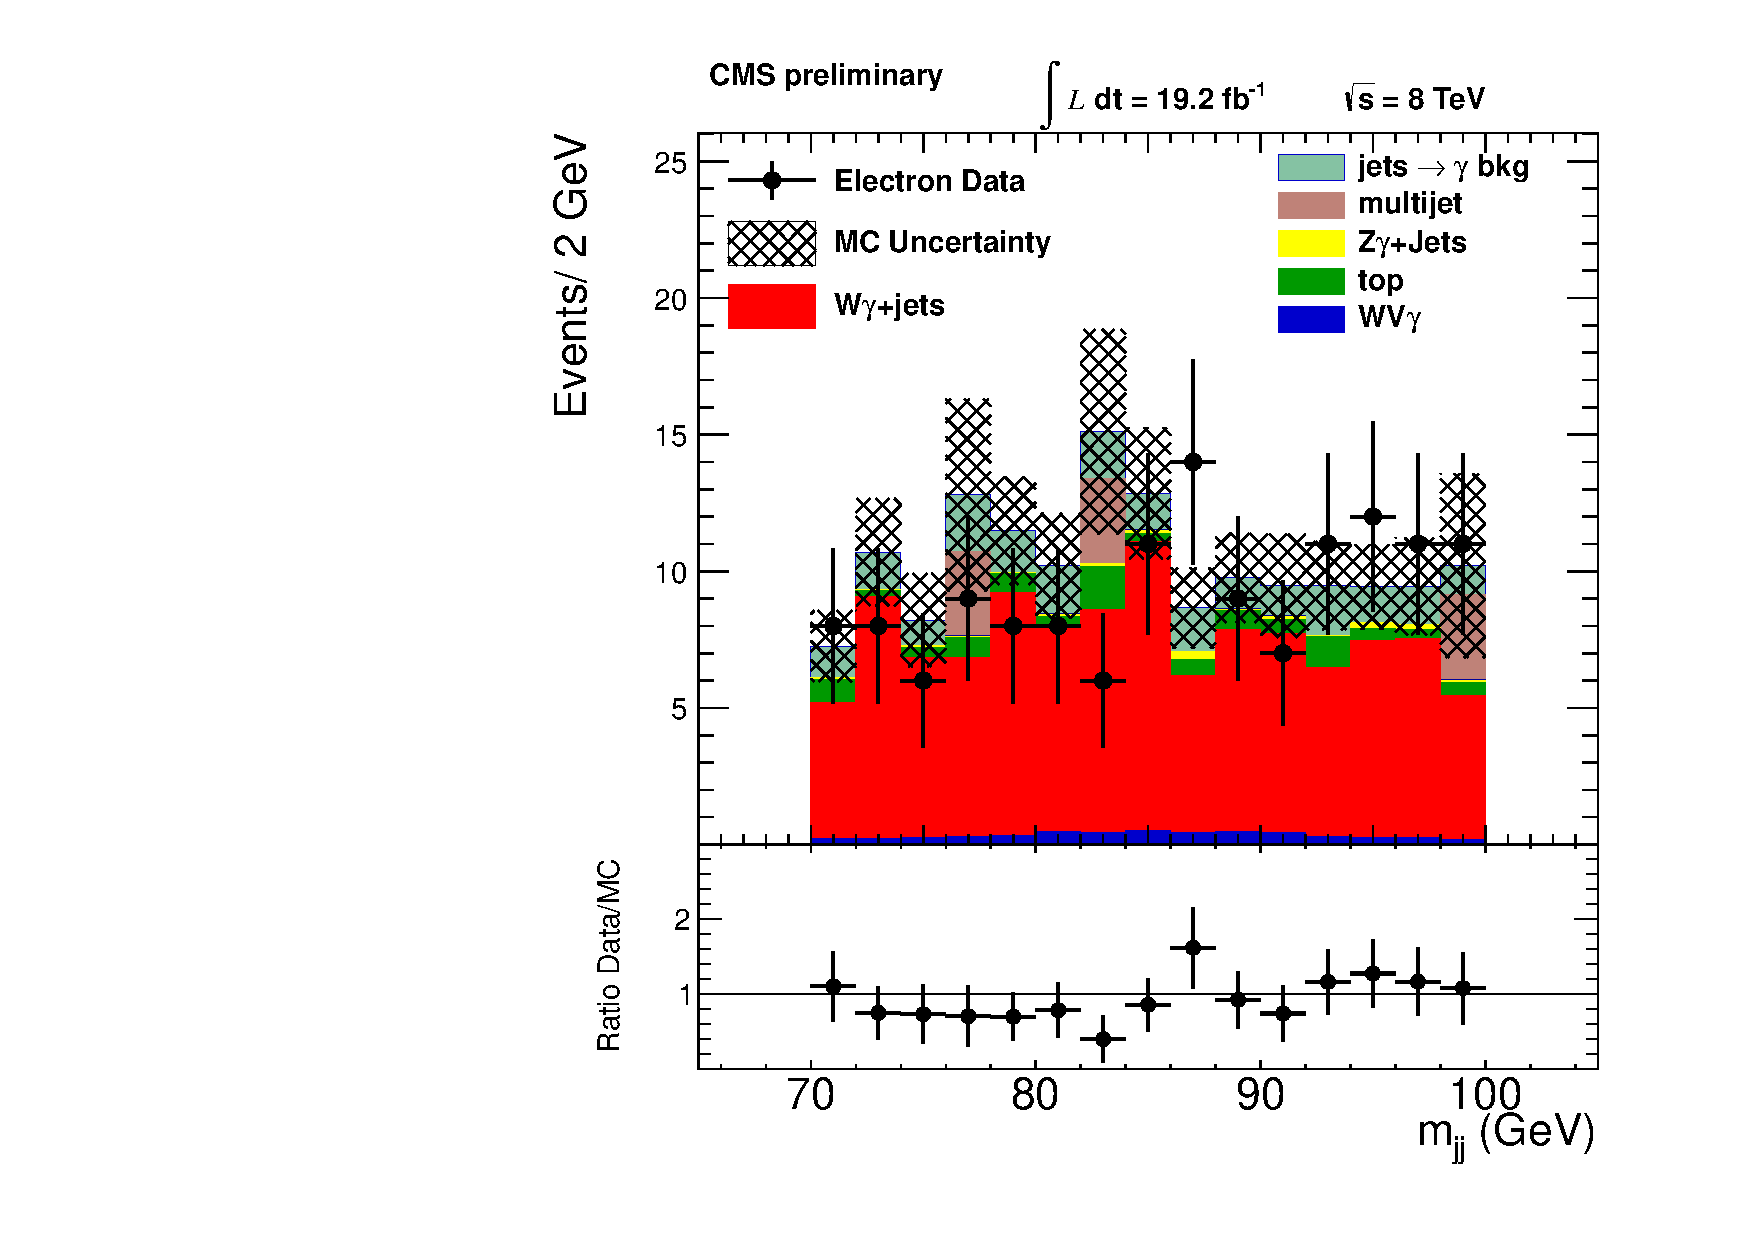
\includegraphics[width=.32\textwidth]{figs/el_mjj.pdf}
}   
\caption{Data and MC comparison plots for muon channel leading jet $p_{T}$ (a) second jet $p_{T}$ (b), di-jet mass (c);
muon channel leading jet $p_{T}$ (d) second jet $p_{T}$ (e) and di-jet mass (f)}
\label{mudijetplots}
\end{center}
\end{figure}

\begin{figure}[b]
\begin{center}
\subfigure[]{
   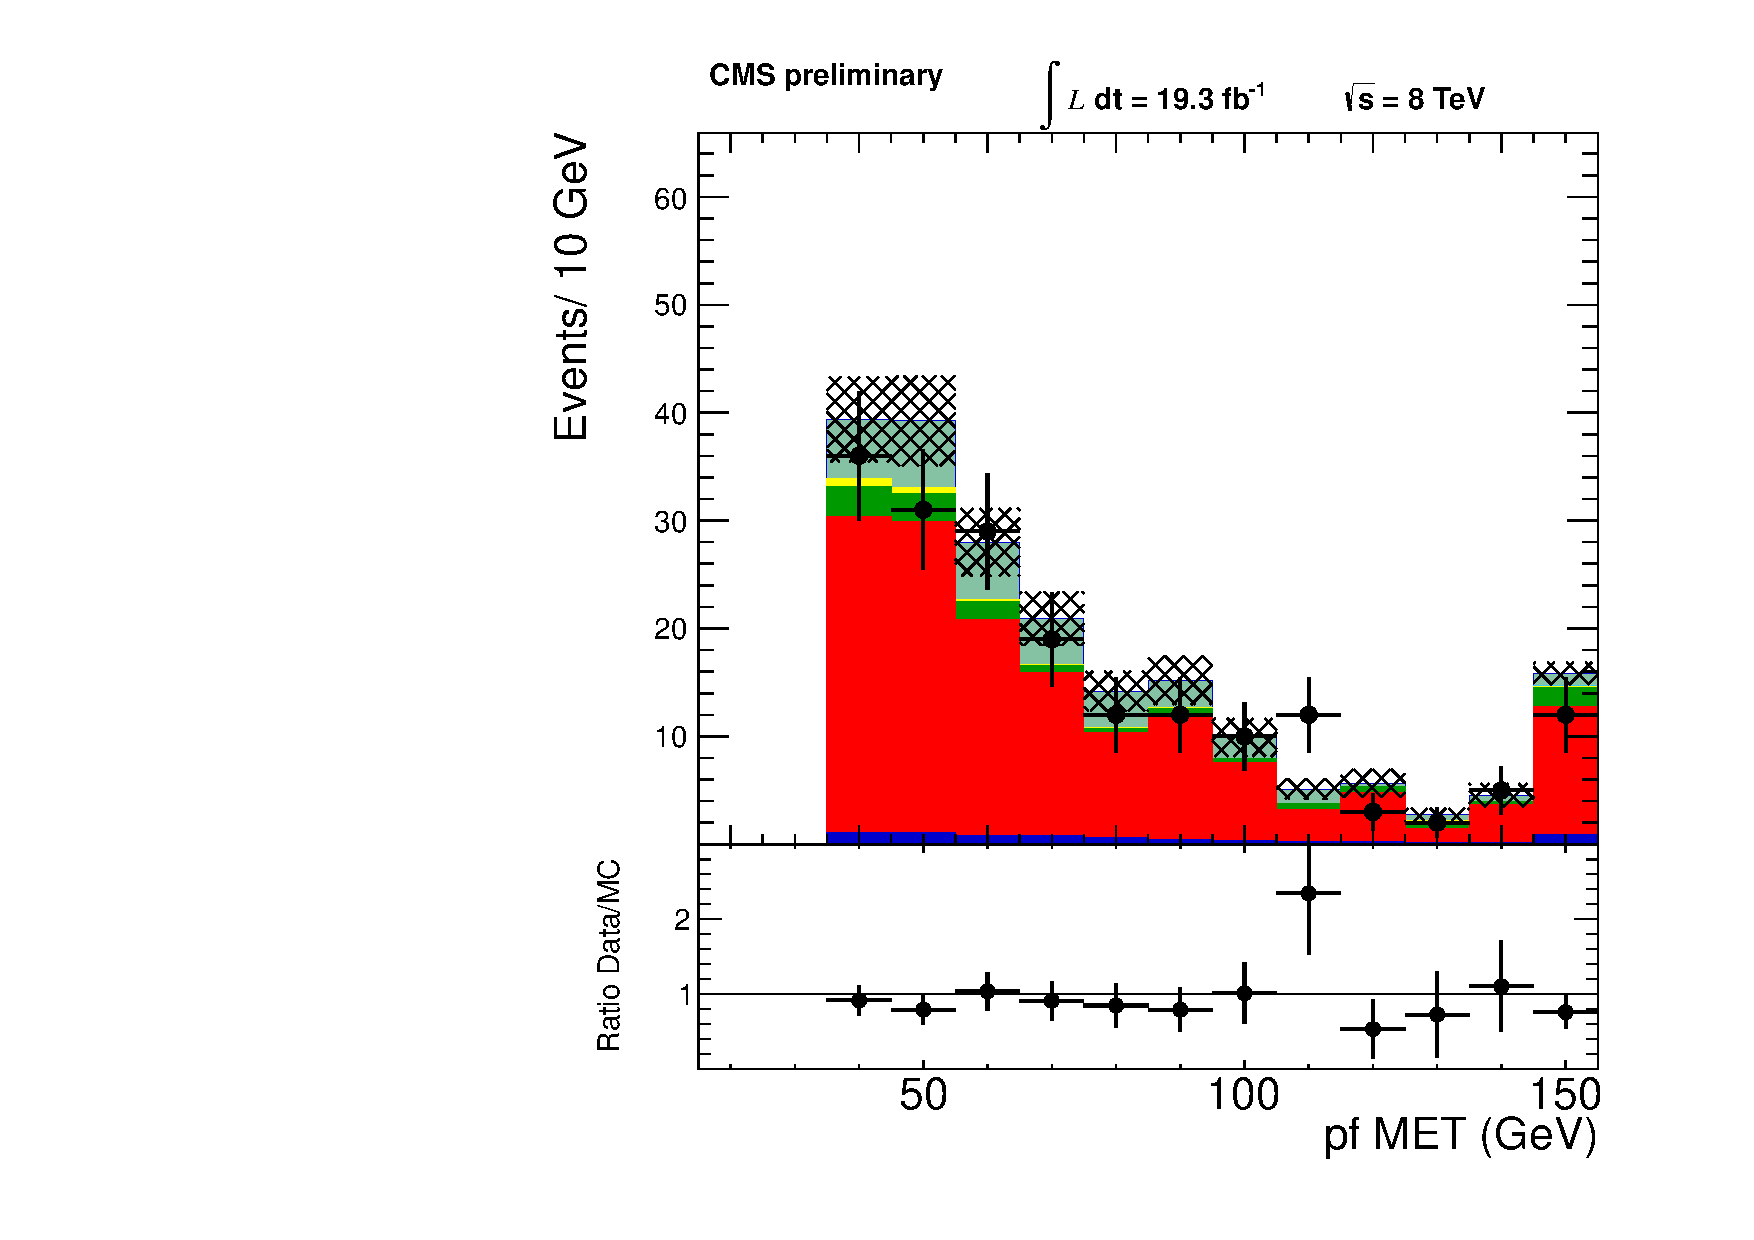
\includegraphics[width=.32\textwidth]{figs/mu_event_met_pfmet.pdf}
}   
%\subfigure[]{
%   \includegraphics[width=.32\textwidth]{figs/mu_W_mt1.pdf}
%}   
\subfigure[]{
   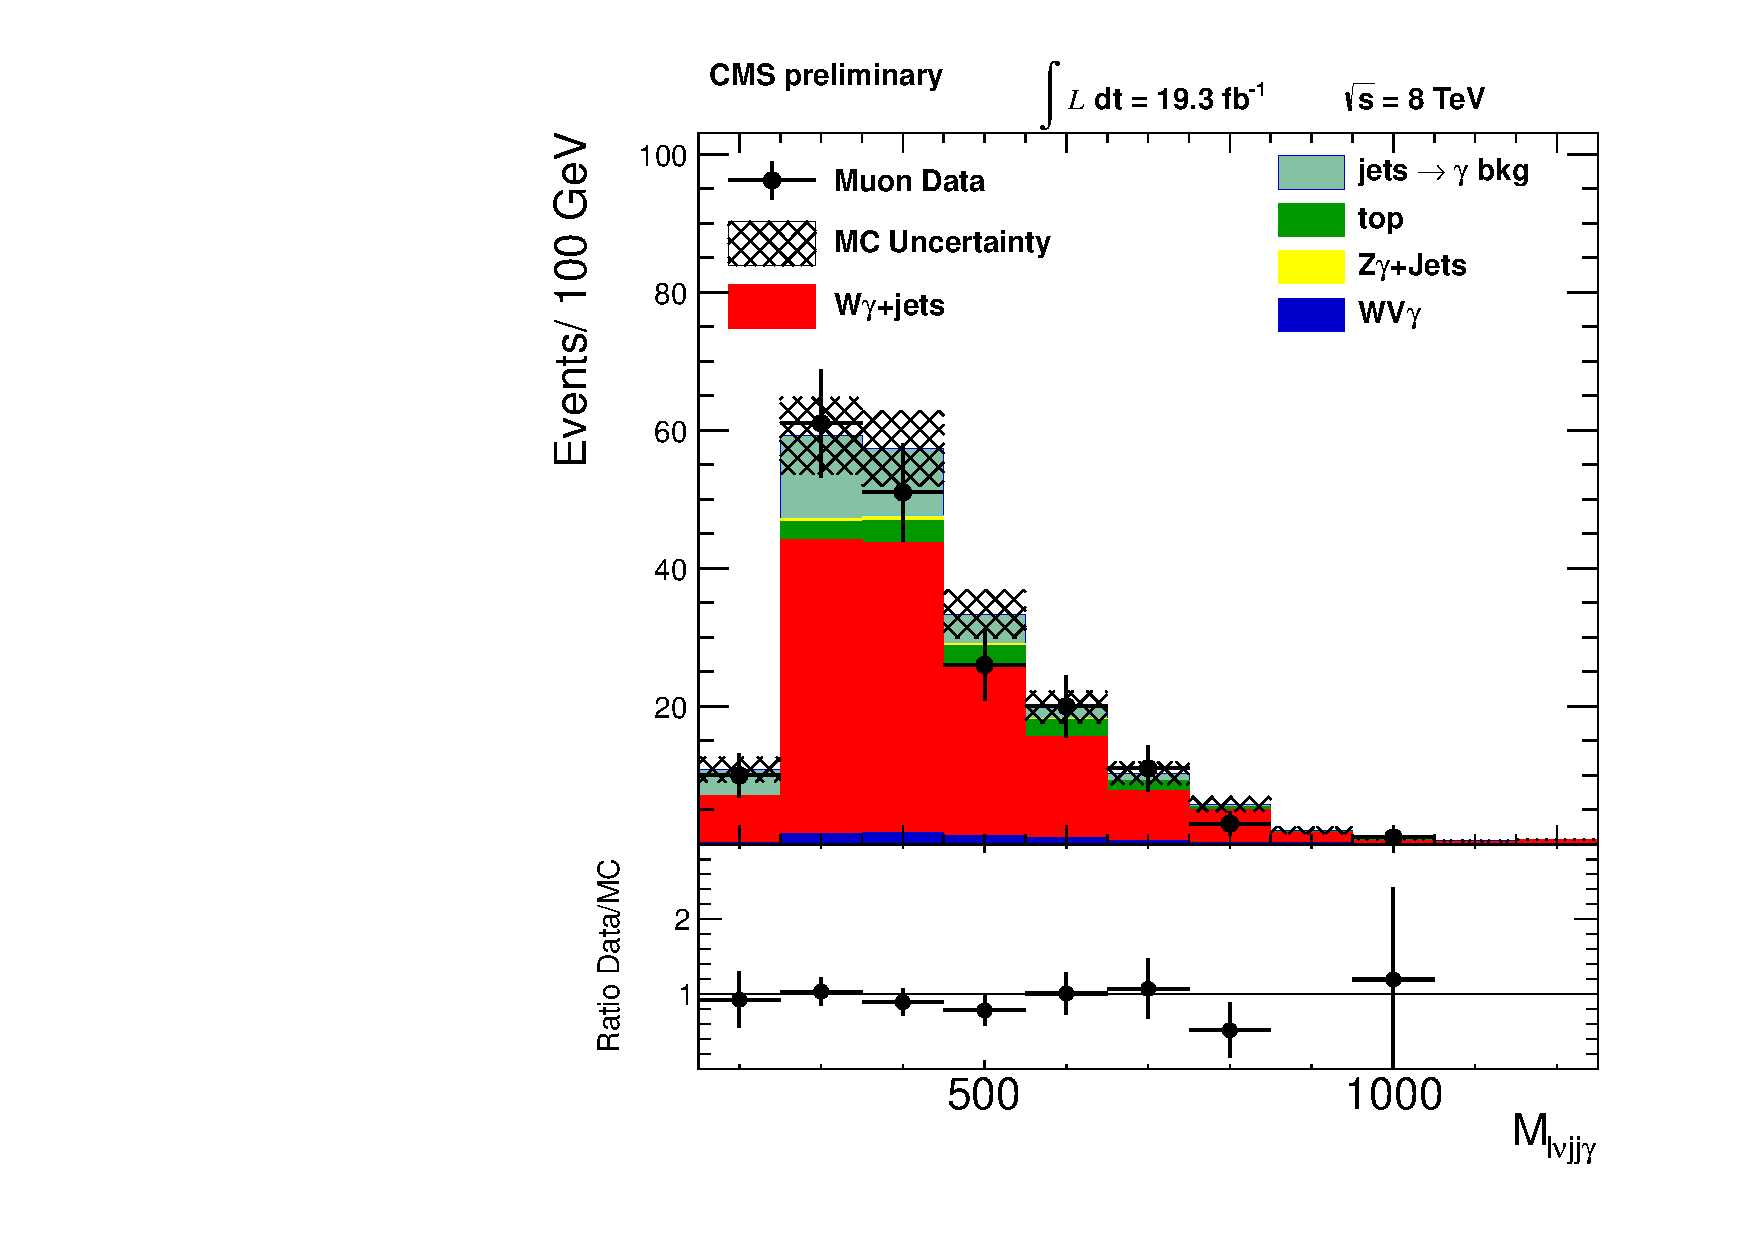
\includegraphics[width=.32\textwidth]{figs/mu_mlvjja1.pdf}
}   \\
\subfigure[]{
   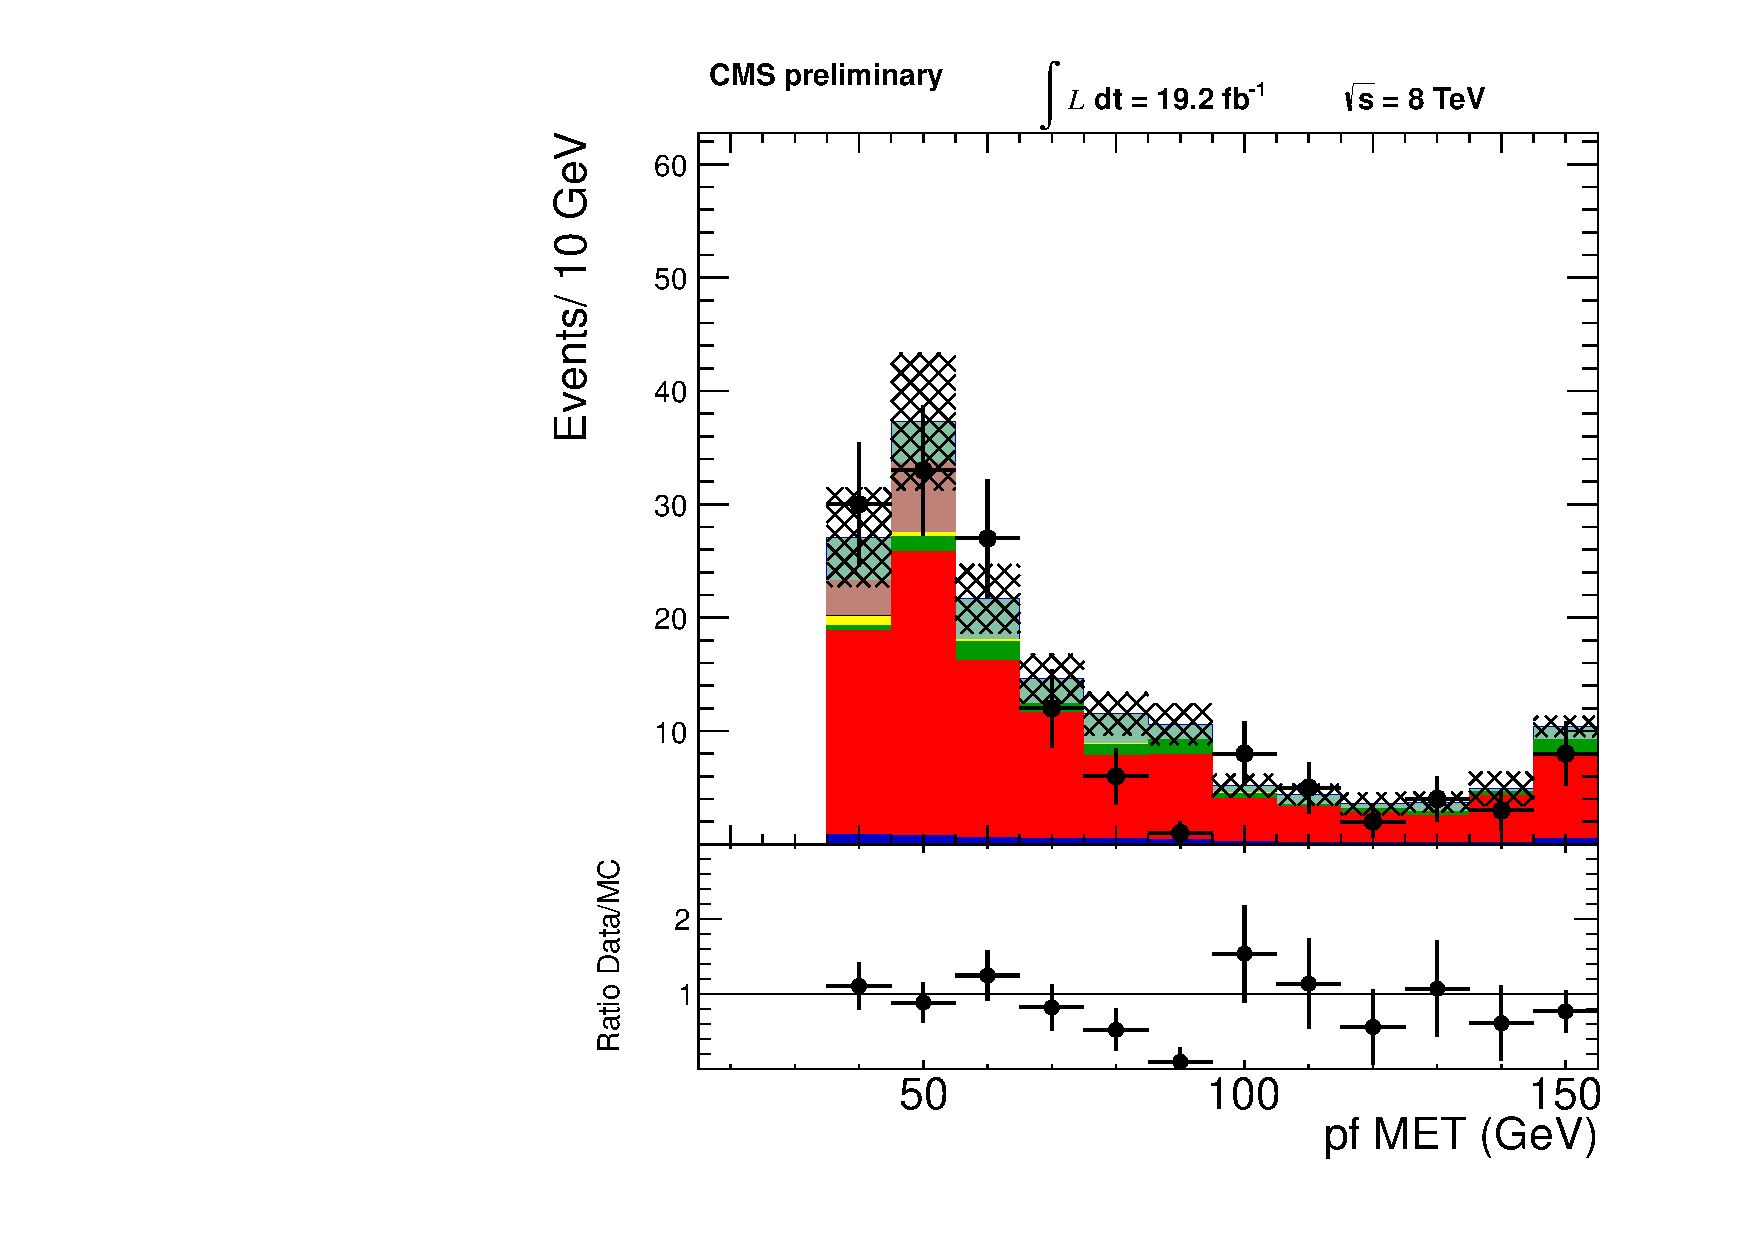
\includegraphics[width=.32\textwidth]{figs/el_event_met_pfmet.pdf}
}   
%\subfigure[]{
%   \includegraphics[width=.32\textwidth]{figs/el_W_mt1.pdf}
%}   
\subfigure[]{
   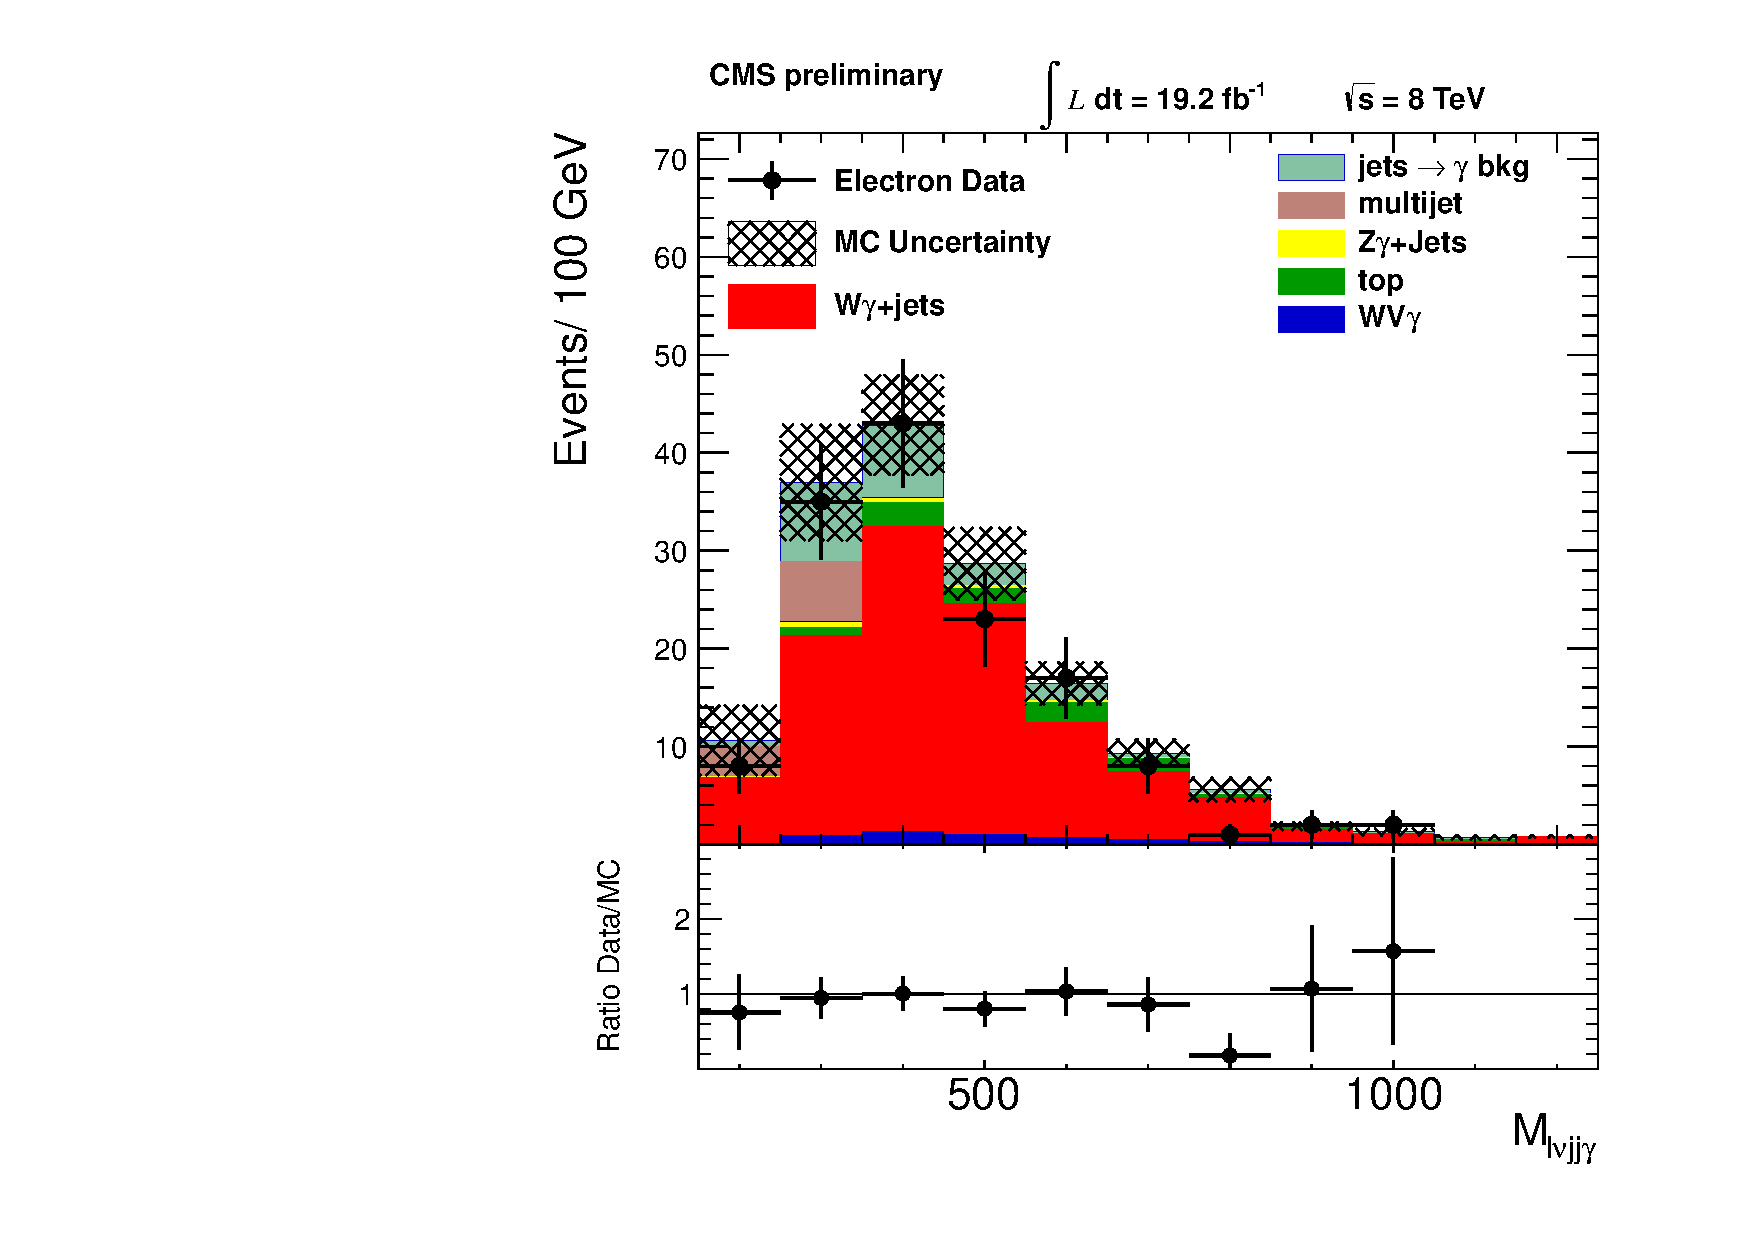
\includegraphics[width=.32\textwidth]{figs/el_mlvjja1.pdf}
}   
\caption{Data and MC comparison plots for muon channel \MET (a)  $M_{lvjj\gamma}$ (b);
electron channel \MET (c) $M_{lvjj\gamma}$ (d)}
\label{eldijetplots}
\end{center}
\end{figure}

Event yield is summarized in Table \ref{tab:evt}.

\begin{table}[htb]
\centering
\scalebox{1.15}{
  \begin{tabular}{|c|c|c|}
  \hline
  Process  & muon channel & electron channel  \\
    & number of events & number of events  \\
  \hline
  \hline
  W$\gamma$+jets                   & 136.9 $\pm$ 3.5  $\pm$ 9.2  $\pm$ 0.0  & 101.6 $\pm$ 2.9 $\pm$ 8.0 $\pm$ 0.0  \\
  WV+jet, jet$\rightarrow \gamma$  & 33.1  $\pm$ 1.3  $\pm$ 4.6  $\pm$ 0.0  & 21.3  $\pm$ 1.0 $\pm$ 3.1 $\pm$ 0.0  \\
  MC t$\overline{t}\gamma$         & 12.5  $\pm$ 0.8  $\pm$ 2.9  $\pm$ 0.5  & 9.1   $\pm$ 0.7 $\pm$ 2.1 $\pm$ 0.4  \\
  MC single top                    & 2.8   $\pm$ 0.8  $\pm$ 0.2  $\pm$ 0.1  & 1.7   $\pm$ 0.6 $\pm$ 0.1 $\pm$ 0.1  \\
  MC Z$\gamma$+jets                & 1.7   $\pm$ 0.1  $\pm$ 0.1  $\pm$ 0.1  & 1.5   $\pm$ 0.1 $\pm$ 0.1 $\pm$ 0.1  \\
  multijets                        & $<$0.2$\pm$ 0.0  $\pm$ 0.1  $\pm$ 0.0  & 7.2   $\pm$ 3.6 $\pm$ 3.6 $\pm$ 0.0  \\
  \hline
  SM WW$\gamma$                    & 6.3   $\pm$ 0.1  $\pm$ 1.5  $\pm$ 0.3  & 4.7   $\pm$ 0.1 $\pm$ 1.1 $\pm$ 0.2  \\
  SM WZ$\gamma$                    & 0.6   $\pm$ 0.0  $\pm$ 0.1  $\pm$ 0.0  & 0.5   $\pm$ 0.0 $\pm$ 0.1 $\pm$ 0.0  \\
  \hline
  Total predicted                  & 193.9 $\pm$ 3.9 $\pm$ 10.8  $\pm$ 1.0  & 147.6 $\pm$ 4.8 $\pm$ 9.6 $\pm$ 0.7  \\
  \hline
  \hline
  Data                             & 183                                    & 139     \\
  \hline
  \end{tabular}}
  \caption{Expected number of events per process, with statistical, systematic and luminosity uncertainties quoted.}
  \label{tab:evt}
\end{table}

